\documentclass[a4paper]{article} 
\usepackage{geometry,fancyhdr,caption,subcaption,graphicx,psfrag,amsfonts,textcomp,mathtools,amsmath,hyperref} 

% settings courtesy of http://www.tjansson.dk/?p=419
\usepackage{listings}
\usepackage{color}
\usepackage{textcomp}
\definecolor{listinggray}{gray}{0.9}
\definecolor{lbcolor}{rgb}{0.9,0.9,0.9}
\lstset{
	backgroundcolor=\color{lbcolor},
	tabsize=4,
	rulecolor=,
	language=matlab,
        basicstyle=\scriptsize,
        upquote=true,
        aboveskip={1.5\baselineskip},
        columns=fixed,
        showstringspaces=false,
        extendedchars=true,
        breaklines=true,
        prebreak = \raisebox{0ex}[0ex][0ex]{\ensuremath{\hookleftarrow}},
        frame=single,
        showtabs=false,
        showspaces=false,
        showstringspaces=false,
        identifierstyle=\ttfamily,
        keywordstyle=\color[rgb]{0,0,1},
        commentstyle=\color[rgb]{0.133,0.545,0.133},
        stringstyle=\color[rgb]{0.627,0.126,0.941},
}

\title{Mandatory exercise 4 \\
Signal and Image Processing 2012} 
\author{Jens P. Raaby \\
\url{frn617@diku.dk}}

\begin{document} 
\maketitle

\section*{Question 4.1 - Gamma Correction} To implement the user interface I used the GUIDE tool in Matlab. The image (in the form of an M x N array of pixels) is passed to the tool via an argument, for example 
\begin{lstlisting}
	gammatool(imread('barbara.tif')); 
\end{lstlisting}

The result of loading the tool is shown in the figure \ref{q1demo}, and the source code is listed in appendix \ref{appendix-gammatool}. I set the slider component to take input in the range -1 to 1, which are applied as exponents of 10 to give gamma values in the range 0.1 to 10.
\begin{figure}[h]
	\centering 
	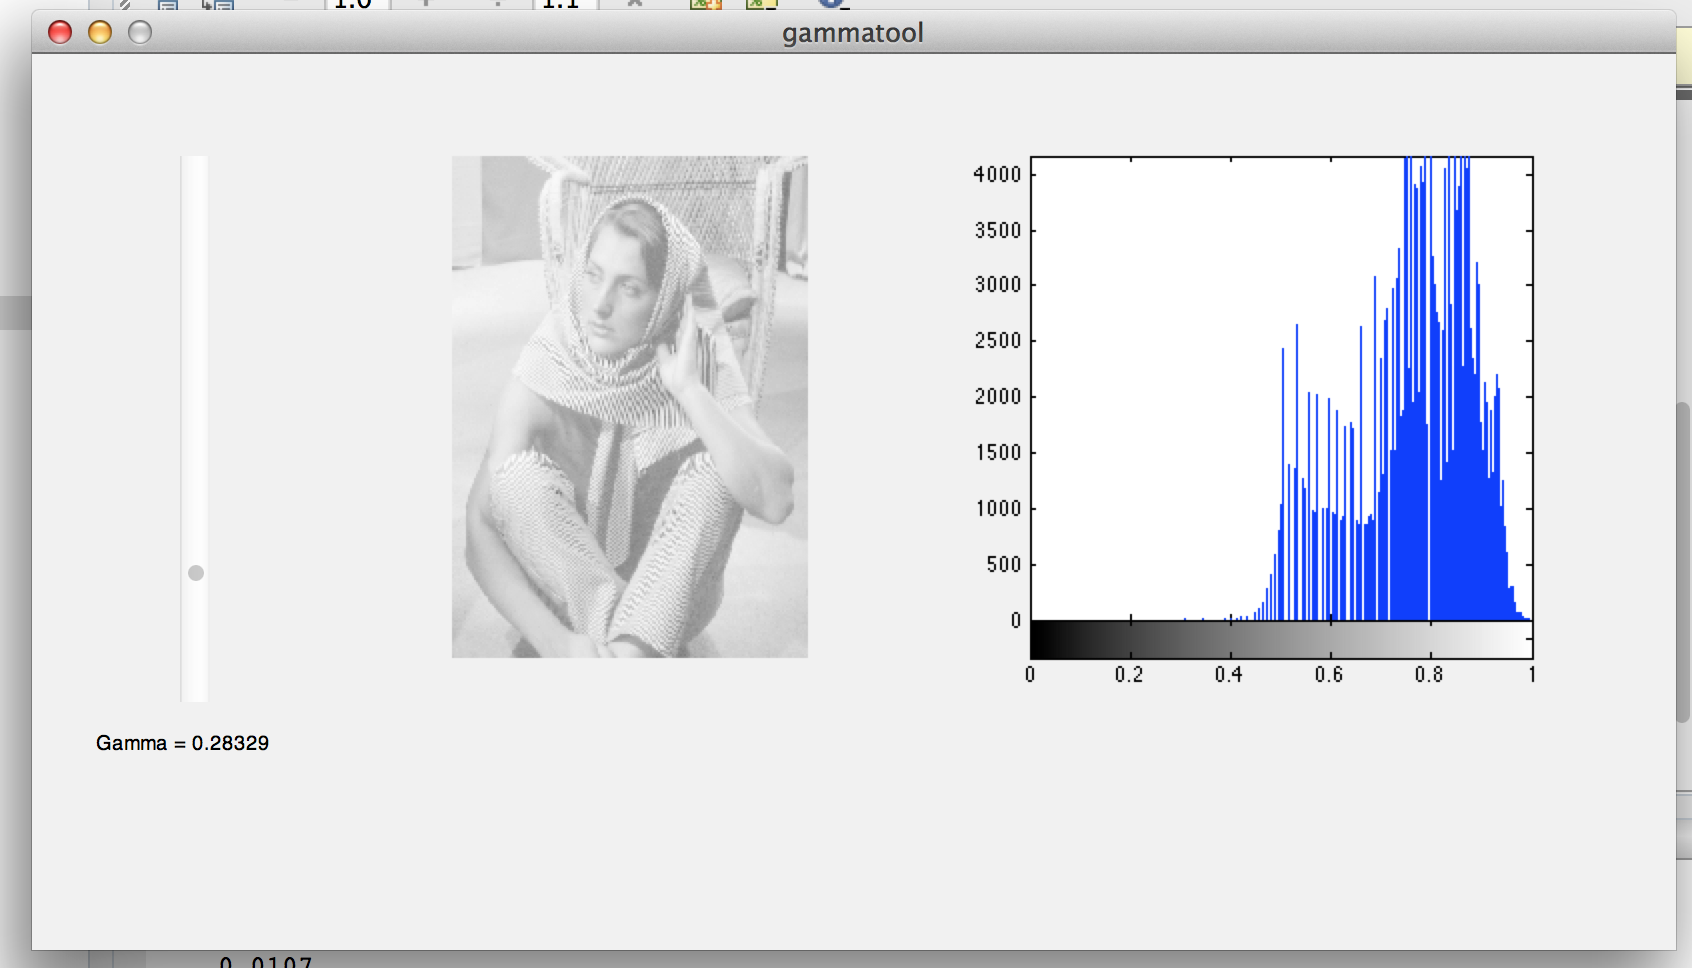
\includegraphics[width=0.7
	\textwidth]{gammatool.png} \caption{Demonstration of the Gamma tool developed for Q4.1} \label{q1demo} 
\end{figure}
\section*{Question 4.2 - Monotonic intensity changes} 
The definition of a strictly decreasing function $g(r)$ is that when $r_2 < r_1$, $g(r_2) < g(r_1)$.
The cumulative probability distribution always sums to 1, but in the decreasing case has the opposite gradient and thus the probability density function is different. When the function $g$ is strictly decreasing and has an inverse, then that inverse function is also decreasing.

The domain and range of the inverse function can thus be expressed:
\begin{equation}
	g^{-1}(( -\infty, s]) = [g^{-1}(s),\infty)    
\end{equation}
Since $s = g(r)$ and $r = g^{-1}(s)$, 
\begin{equation}
    P_S(s) = P(R \in [g^{-1}(s), \infty))
    \label{PrRange}
\end{equation}

\begin{equation}
    P_S(g(r)) = P_R(r) \Leftrightarrow P_S(s) = P_R(g^{-1}(s))
    \label{PsPr}
\end{equation}

We have the definition of $P_R(t)$ (it always takes value 1), and since we know the integration intervals in this decreasing case from above:
\begin{equation}
    P_R(t) = \int_t^\infty p_r(x) dx + \int_{-\infty}^t p_r(x) dx = 1
    \label{sumint}
\end{equation}
\begin{equation}
    P_R(t) = \int_{-\infty}^\infty p_r(x) dx = 1
\end{equation}
Hence from (\ref{PsPr}) and (\ref{sumint}):
\begin{equation}
    P_S(t) = 1 - P_R(t) = 1 - P_R(g^{-1}(s))
\end{equation}
This follows because $P_R$ can be expressed as the sum of the two integrals, and it always takes value 1. Since we know $P_R$ is the integral of a decreasing function, and we know its range from (\ref{PrRange}), then this is rearranged as $1 - P_R(t)$.

Now the derivatives can be calculated:

\begin{equation}
\frac{d(P_S(t))}{dr} = \frac{d(P_S(g(r)))}{dr} = \frac{d(1-P_R(r))}{dr} 
\end{equation}
Beginning with the right hand side:
\begin{equation}
     \frac{d(1-P_R(r))}{dr} = -p_R(r)
\end{equation}
The left side can be derived using the chain rule:
\begin{equation}
    \frac{d(P_S(g(r)))}{dr} = p_S(s) \frac{d(g(r))}{dr} = p_S(s)\frac{ds}{dr} = -p_R(r)
\end{equation}

\begin{equation}
g'(s) = \frac{ds}{dr} = \frac{-p_R(r)}{p_S(s)}
\end{equation}
\begin{equation}
g'(s) = \frac{-p_R(r)}{p_S(g(r))}
\end{equation}
This is the complement of the equation given in the slides for a strictly increasing intensity change. The general formulation for a strictly monotonic intensity change is thus the:
\begin{equation}
    g'(s) = |{\frac{ p_R(r) }{p_S(g(r))}}|
\end{equation}
In other words, the derivative of $g(s)$ is the probability density function of the input divided by the probability density function of the transformed input, and it will take a negative value if the change is monotonically decreasing, positive if increasing.

%%%%%%%%%%%%%%%%%%%%%
\section*{Question 4.3}
We have the function over the interval $R \in [0,1]$:
\begin{equation}
    g(r) = \frac{1}{2}(1+cos(2\pi r))
    \label{eq:43}
\end{equation}
\begin{figure}[t]
    \centering

    \begin{subfigure}[b]{0.4\textwidth}
            \centering
            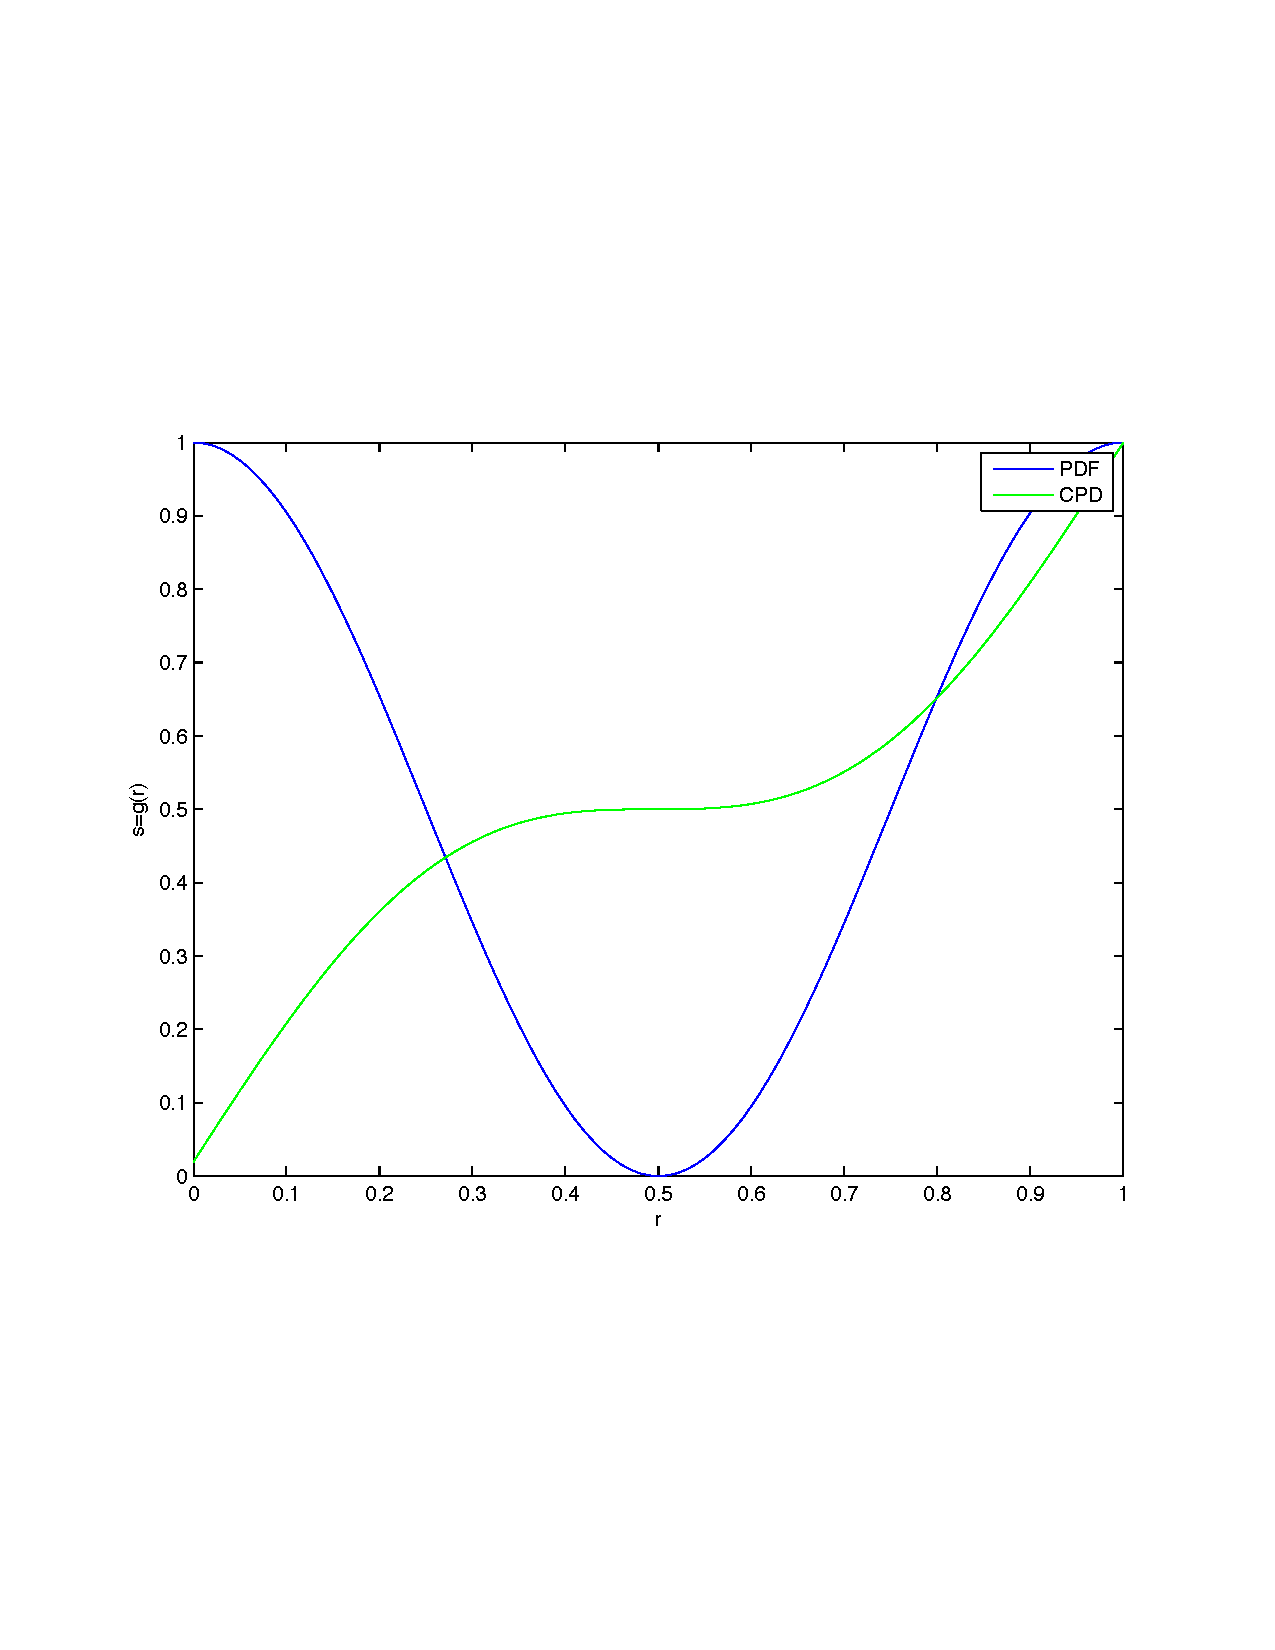
\includegraphics[width=\textwidth]{q3-plot.pdf}
            \caption{Plot of $g(r)$ and its CPD}
            \label{fig:43plot}
    \end{subfigure}\quad
    \begin{subfigure}[b]{0.4\textwidth}
            \centering
            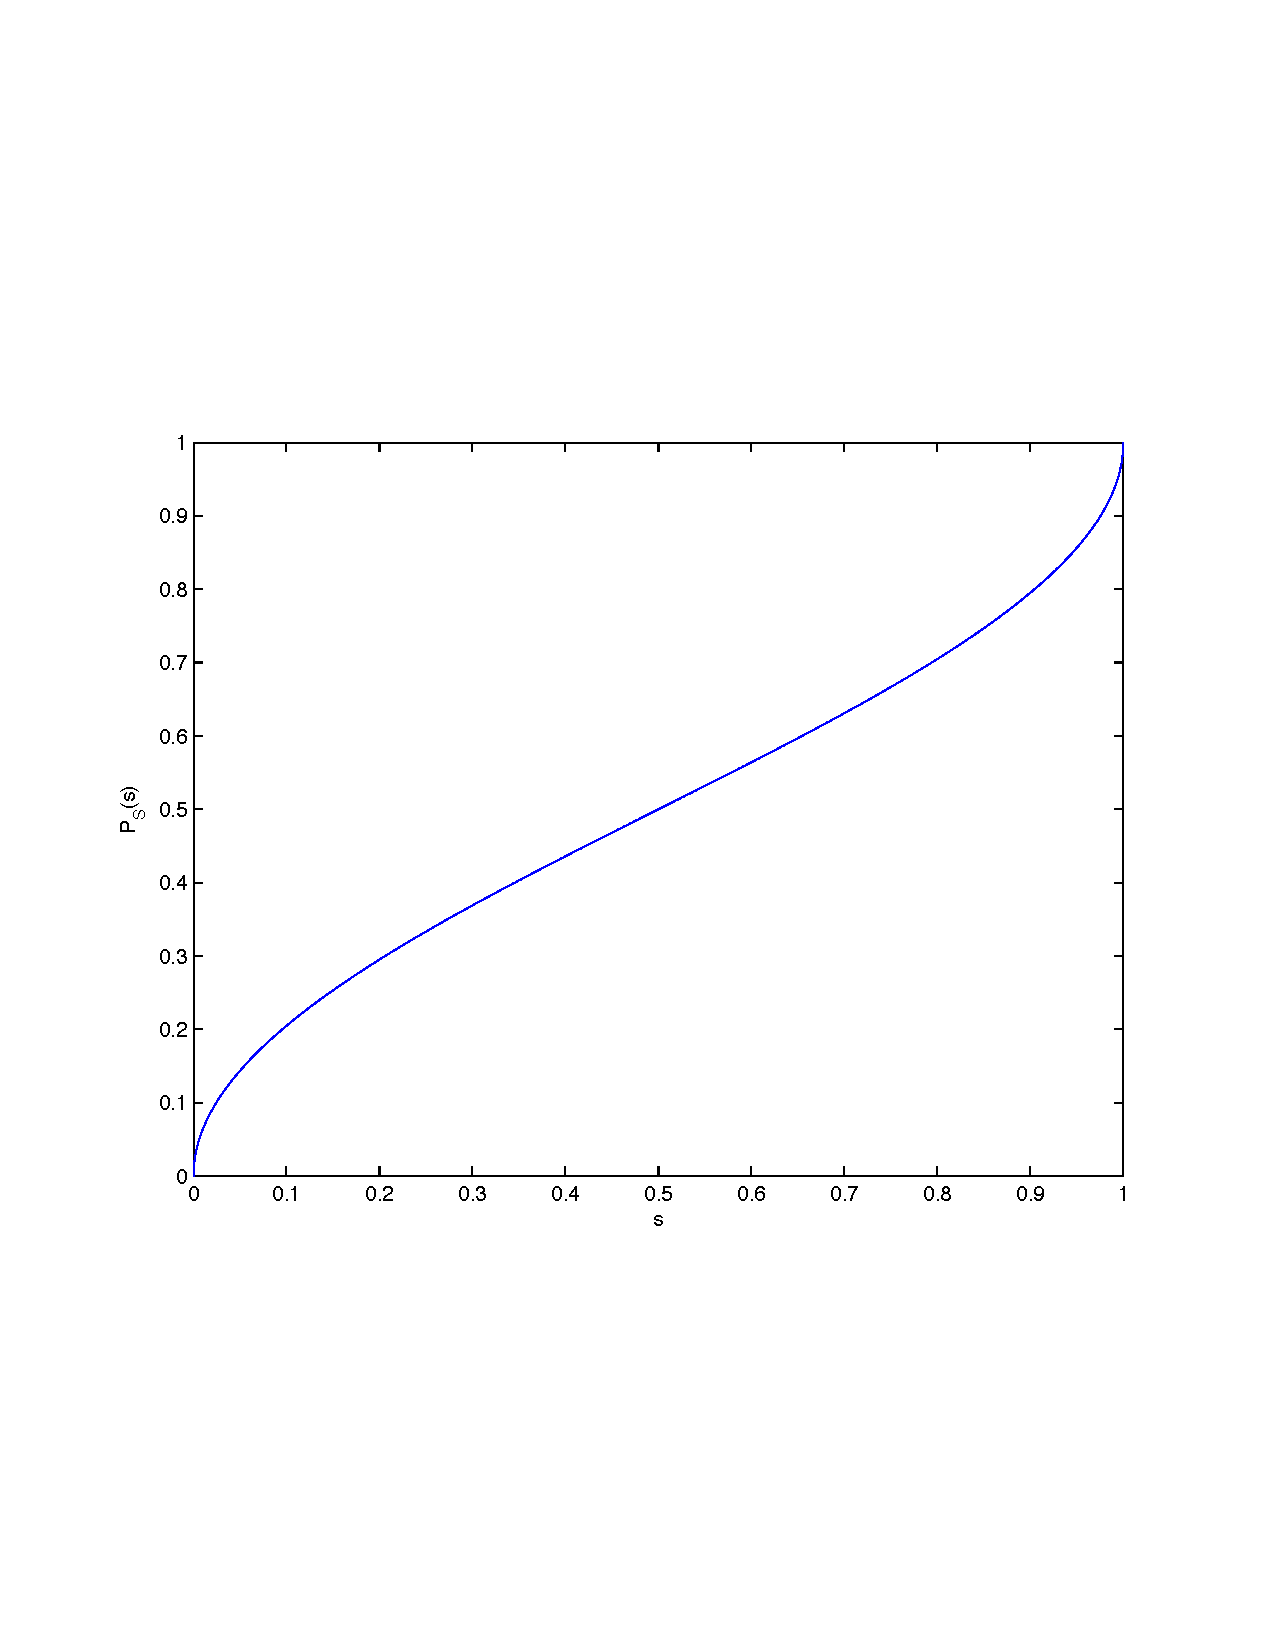
\includegraphics[width=\textwidth]{q3-cpds}
            \caption{CPD of $S$, $P_S(s)$}
            \label{fig:43cpds}
    \end{subfigure}
    \caption{Plots for question 4.3}
    \label{fig:43plots}
\end{figure}
To find the CPD of S in terms of the CPD of R, (\ref{eq:43}) must be rearranged in terms of $r$:
\begin{eqnarray}
    && s = g(r) = \frac{1}{2}(1+cos(2\pi r))\\
    && 2s = 1+cos(2\pi r)\\
    && 2s - 1 = cos(2\pi r)\\
    && cos^{-1}(2s - 1) = 2\pi r\\
    && r = \frac{cos^{-1}(2s - 1)}{2\pi}
    \label{eq:43r}
\end{eqnarray}
In the given interval, this gives 2 roots, given some value for s. This can be inferred by inspecting the graph of $g(r)$ in figure \ref{fig:43plot}. Hence the next step is to determine these roots, $r_1$ and $r_2$, in terms of $s$.

The two roots $r_1$, $r_2$ are separated by the symmetry of the PDF around value $r=0.5$.
$r_1$ is given by (\ref{eq:43r}), and $r_2$ is the symmetric case:
\[
r_2 = \frac{2\pi - cos^{-1}(2s - 1)}{2\pi} = 1 - \frac{cos^{-1}(2s - 1)}{2\pi}
\]
This is essentially a `shift' of $r_1$ (the period of the function is 1, and of $cos$ is $2\pi$).

In order to express the cumulative probability distribution of $S$ in terms of the CPD of $R$, the set notation is used for the intermediate steps below:
\begin{eqnarray}
    P_S(s) && =  P(S \leq s)\\
           && =  P(\{\omega | S(\omega) \leq s\})\\
           && =  P(\{\omega | g(R(\omega)) \leq s\})\\ 
           && =  P(\{\omega | g(R(\omega)) \in [r_1,r_2]\})\\ 
           && =  P(\{\omega | g(R(\omega)) \in [\frac{cos^{-1}(2s - 1)}{2\pi},1 - \frac{cos^{-1}(2s - 1)}{2\pi}]\})\\   
           && =  P(\{\omega | g(R(\omega)) \leq \frac{cos^{-1}(2s - 1)}{2\pi}\}) \cap P(\{\omega | g(R(\omega)) \leq \frac{1-cos^{-1}(2s - 1)}{2\pi}\})\\
           && = P_R(1-\frac{cos^{-1}(2s - 1)}{2\pi}) - P_R(\frac{cos^{-1}(2s - 1)}{2\pi})
           \label{eq:43cpd1}
\end{eqnarray}
Note that this indicates that $P_S(s)$ is zero when $P_R(r_2)=P_R(r_1)$.
The result of plotting $P_S(s)$ is shown in figure \ref{fig:43cpds}.


\subsection*{Comparing the results}
In figure \ref{fig:43compare} the intensity transformation $g(r)$ was applied to an image containing a (dithered) linear gradient from white to black. The histograms are shown below. Comparing the histogram afterwards (figure \ref{fig:ah}) to the CPD of the function (shown in figure \ref{fig:43cpds}) shows a similar straight section in the mid-tones of the image. The low and high tones (close to 0 and 1) in the transformed histogram are similar to the original histogram (i.e. higher intensity than the mid-tones). What is interesting from observing the image itself is that the midtones have been dropped towards black, and the dark tones have been boosted/swapped for white (figure \ref{fig:ai}). This correlates with the shape of the function $g(r)$ shown in the blue plot in rigure \ref{fig:43plot}; the light tones ($r$ near 1) are not significantly changed.

The CPD $P_S$ is characterised by the predominantly flat central section with a steeper gradient close to the limits (0,1). The transformed histogram is also characterised by an almost linear central section with steep gradients towards the end. The central region is less dense than the original image's histogram, because the midtones have been altered by the transformation - they still remain present because there is still a gradient visible in the image, but it is a steeper change in tone (so there are gaps in the histogram).

%\begin{figure}[h]
%    \centering
%    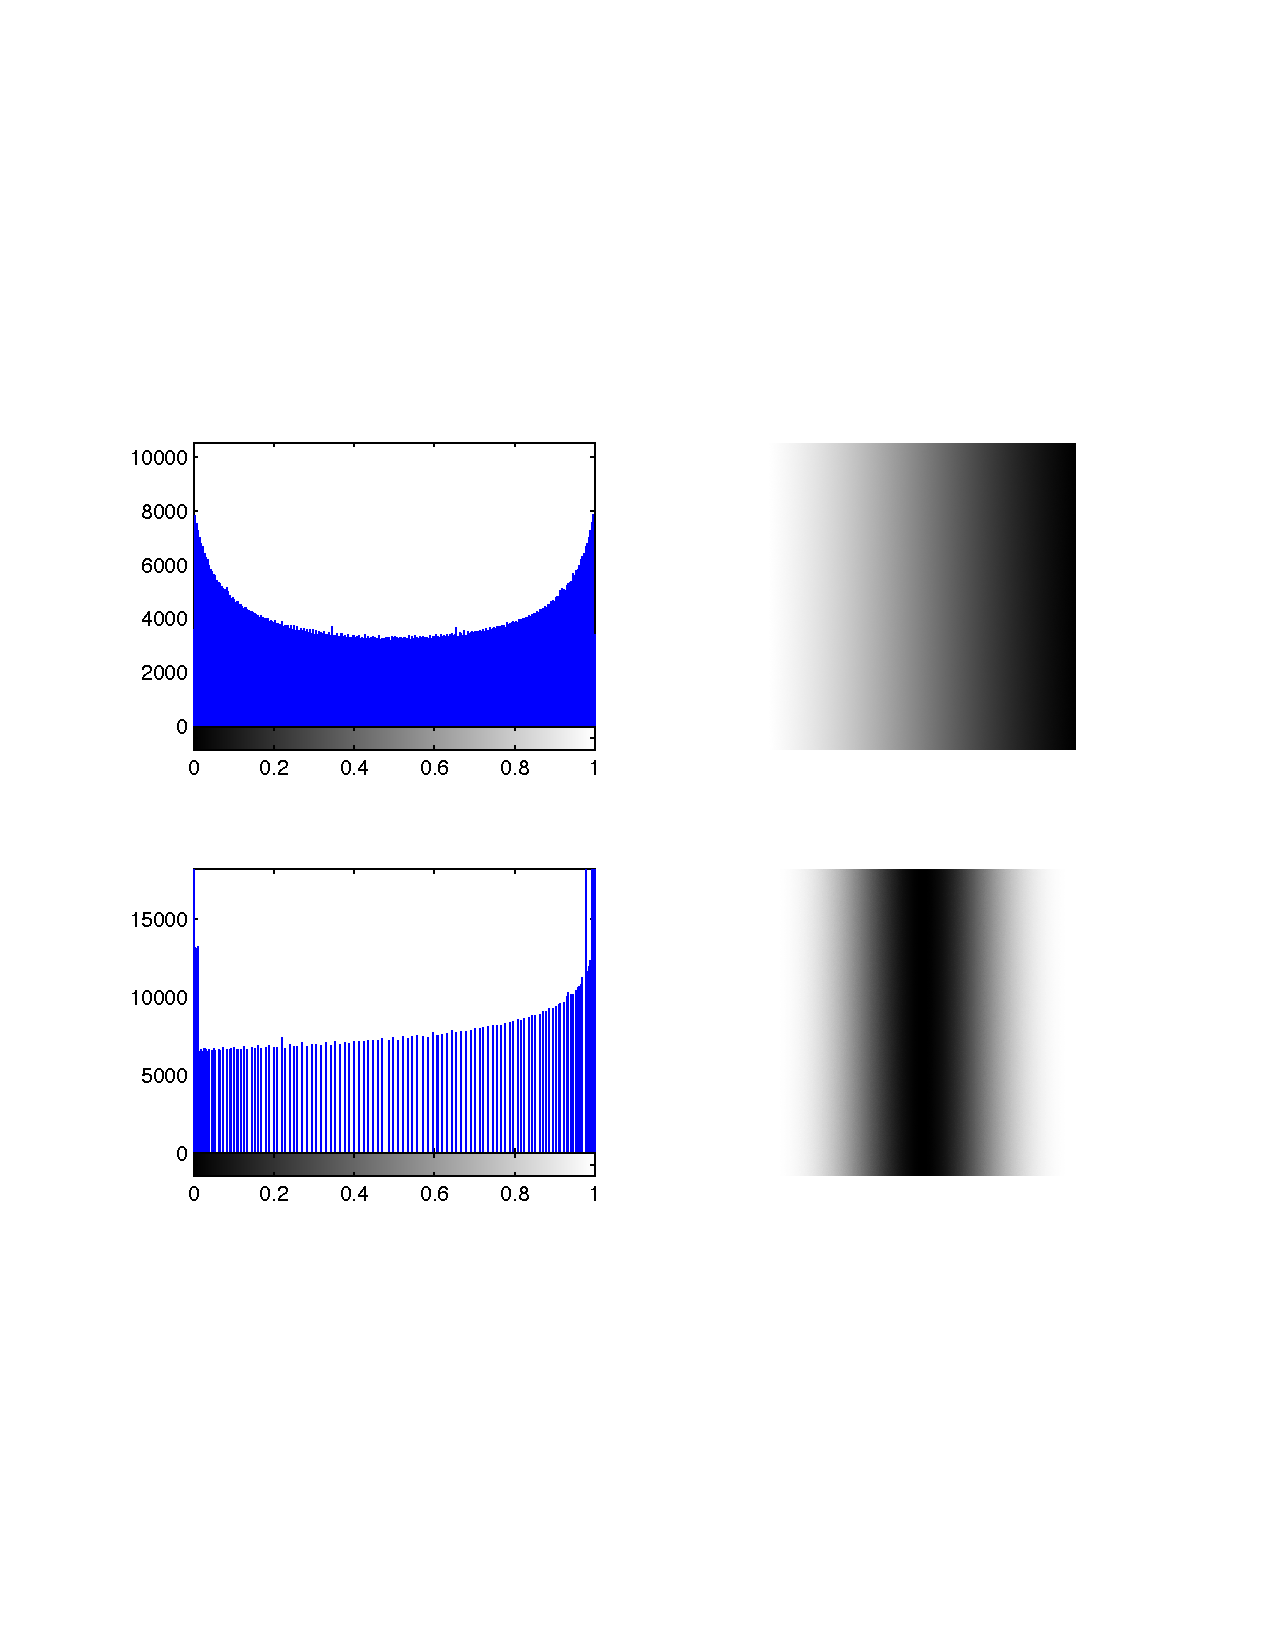
\includegraphics[width=0.9\textwidth]{q3-compare.pdf}
%    \caption{Question 4.3 - image transformed with g(r)}
%    \label{fig:43cmp}
%\end{figure}
\begin{figure}[h!]
        \centering
        \begin{subfigure}[b]{0.3\textwidth}
                \centering
                
\includegraphics[width=\textwidth]{q3-beforeim.png}
                \caption{Input image}
                \label{fig:bi}
        \end{subfigure}
        \begin{subfigure}[b]{0.3\textwidth}
                \centering
                
\includegraphics[width=\textwidth]{q3-afterim.png}
                \caption{Image after g applied}
                \label{fig:ai}
        \end{subfigure}
        
        \begin{subfigure}[b]{0.3\textwidth}
                \centering
                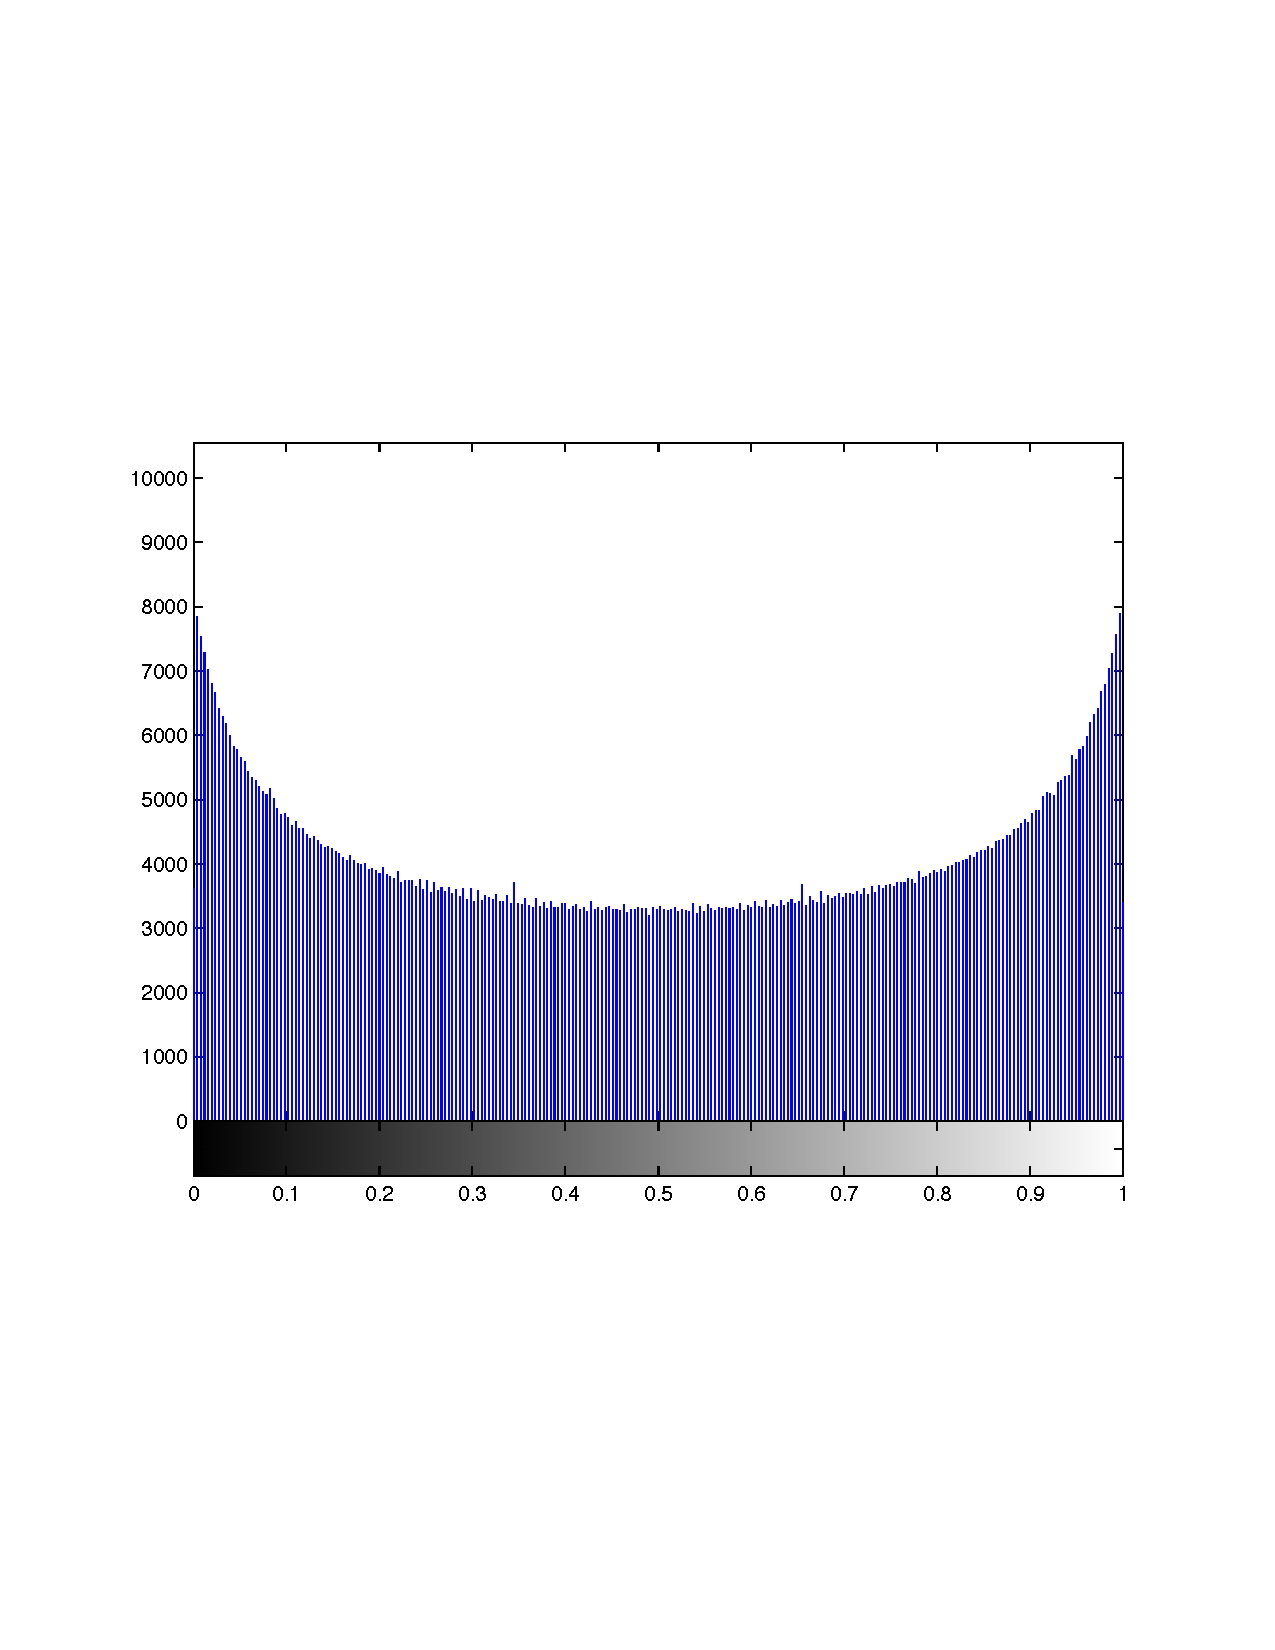
\includegraphics[width=\textwidth]{q3-beforehist}
                \caption{Histogram of original image}
                \label{fig:bh}
        \end{subfigure}%
        ~ %add desired spacing between images, e. g. ~, \quad, \qquad etc. 
          %(or a blank line to force the subfigure onto a new line)
        \begin{subfigure}[b]{0.3\textwidth}
                \centering
                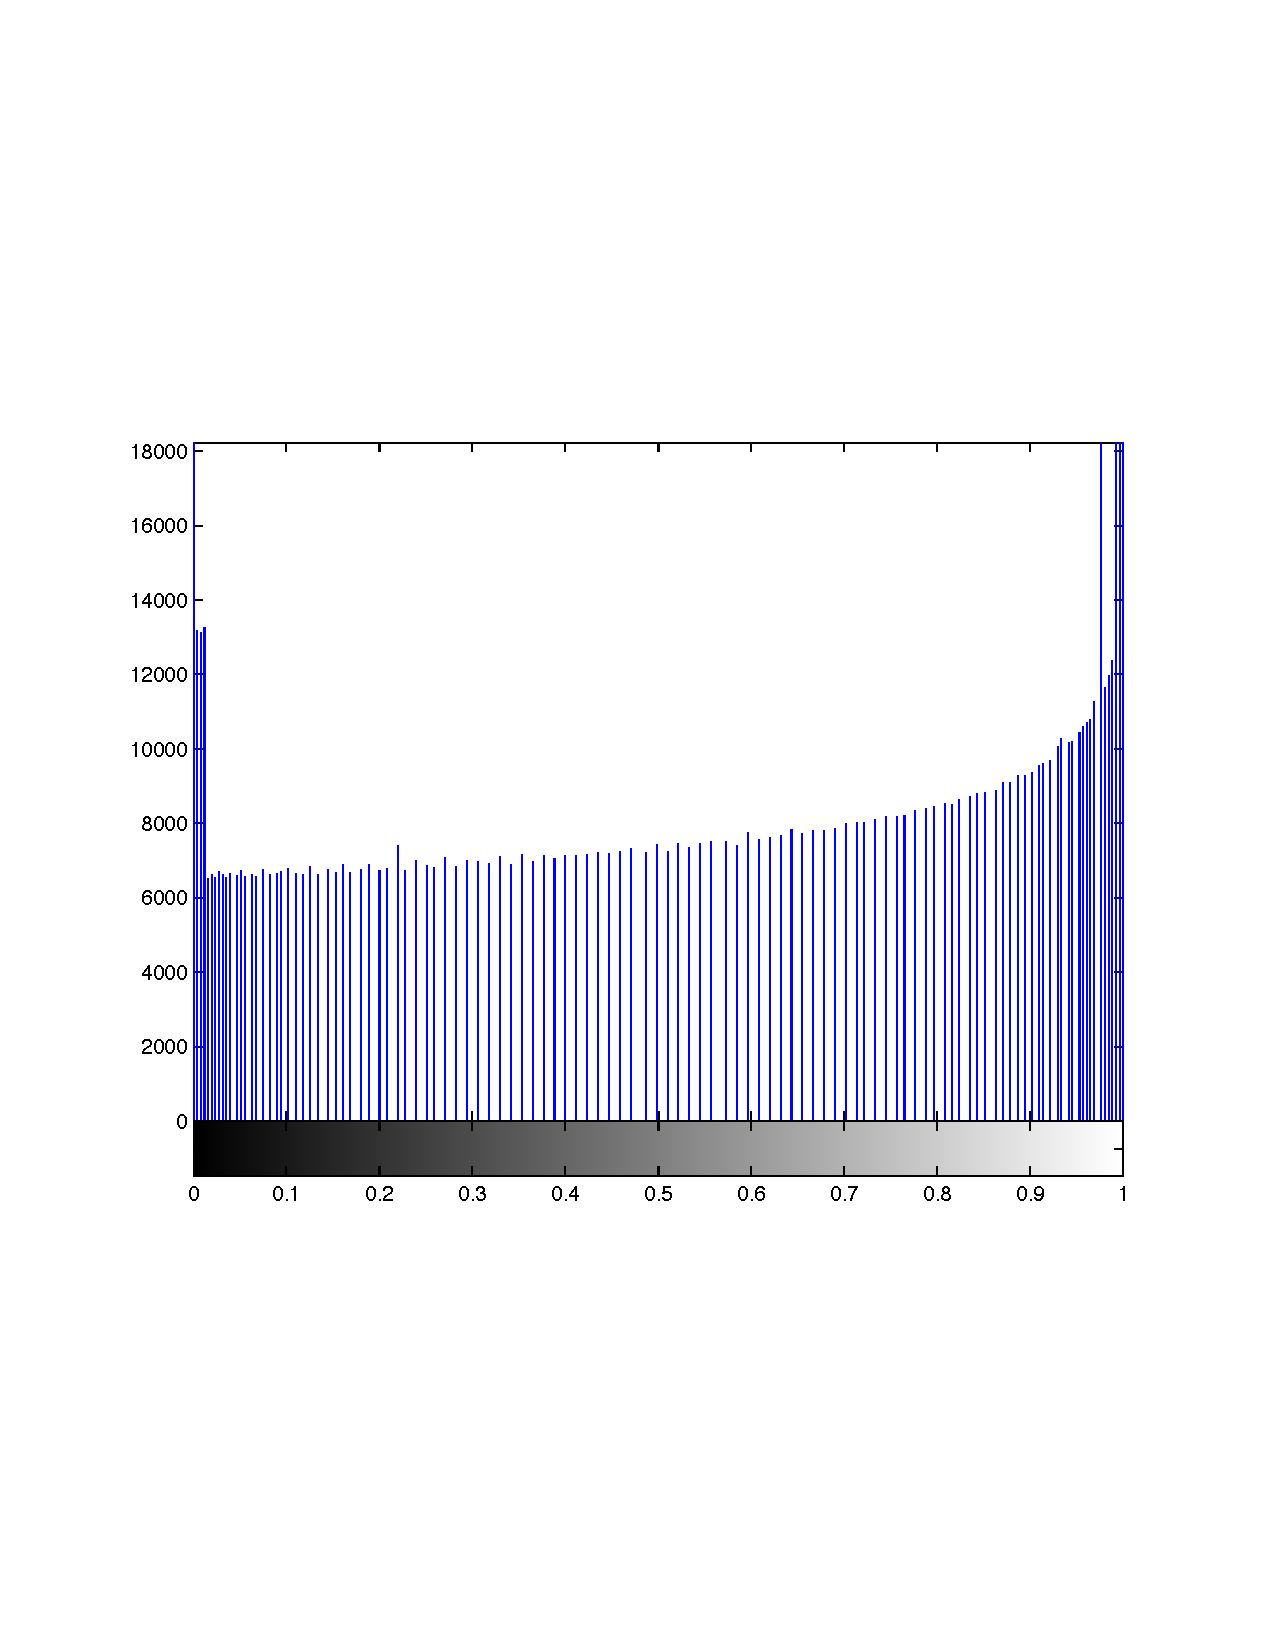
\includegraphics[width=\textwidth]{q3-afterhist}
                \caption{Histogram after $g$ applied}
                \label{fig:ah}
        \end{subfigure}
        \caption{Results of applying $g$}\label{fig:43compare}
\end{figure}


\section*{Question 4.4 - Histogram equalisation and matching} 
Histogram equalisation is applied by the function histogram\_equalise(image) defined in histogram\_equalise.m (see appendix \ref{appendix-hist-eq}).

The equalisation method involves non-whole nubers, because the CPD is calculated (and it is a sum of probabilities and therefore a fraction at each point in the range $(0,1)$). These must be quantized back to integers in the equalised image and therefore some of the information will be lost. There is not an obvious way to remove this problem. One workaround could be to extend the range of intensities to 16 bit rather than 8 bit, but a lot of display hardware cannot show this many intensity levels. Another possible method to improve the situation would be to smooth the histogram of the original image (perhaps by blurring slightly) to give a more continuous input PDF. There would still be some rounding error but spikes in the histogram would be less likely.

The images in figure \ref{fig:441compare} show the result of histogram equalisation on the `Barbara' image. It is clear from the histograms that the equalised image has a more spread out range of intensities, but the pattern is not perfectly uniform, and both gaps and spikes are exaggerated by the transformation.

Histogram matching is defined in histogram\_match.m, as listed in appendix \ref{appendix-hist-match}. 

The potential problems caused by quantization include matching an image to a histogram which is not monotonic in its intensity changes. The result is that there is not a 1-1 mapping between an intensity on the matched image and one in the original image (in other words, the matching has compressed the data). This also means it is not possible to restore the image back to its original intensities accurately, because there will be an ambiguity in the mapping of intensities. 

In my example shown in figure \ref{fig:bhe3}, the start and end of the histogram is almost flat (and thus potentially non-monotonically changing). This means there is an ambiguity in the matching process, and some of the data will be incorrectly mapped and detail lost. The cliff face in the upper middle part of the image in figure \ref{fig:ae2} has less contrast than in the original version, caused by this quantization error.
If any given input intensity matches equally to two or more of the specimen intensities, then a decision must be made. This means that information is essentially lost or corrupted in the transformation. Gonzalez and Woods (page 133) suggest choosing the smallest value by convention. This might be a temporary solution, but is not always ideal.

Images with many pixels with intensities close to zero may have a problem being matched to a specimen histogram (this is the case with my example in figure \ref{fig:be2}). The potential solution is to apply an additional histogram matching operation which smooths the transitions of dark pixels. The matching can be applied after this first transformation. This is the approach explained by Gonzalez and Woods (pp. 137-8).



\begin{figure}[h!]
        \centering
        \begin{subfigure}[b]{0.3\textwidth}
                \centering
                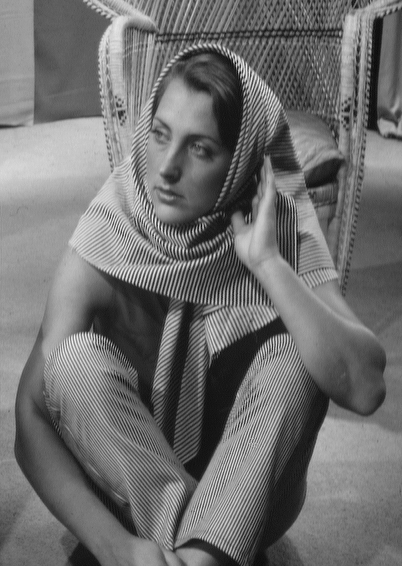
\includegraphics[width=\textwidth]{q4-orig.png}
                \caption{Input image}
                \label{fig:be}
        \end{subfigure}
        \begin{subfigure}[b]{0.3\textwidth}
                \centering
                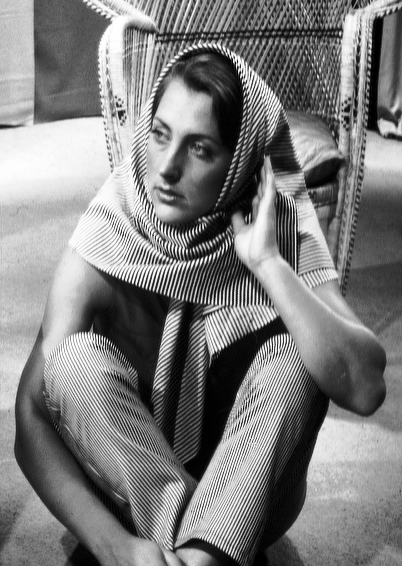
\includegraphics[width=\textwidth]{q4-equal.png}
                \caption{Image after equalisation}
                \label{fig:ae}
        \end{subfigure}
        
        \begin{subfigure}[b]{0.3\textwidth}
                \centering
                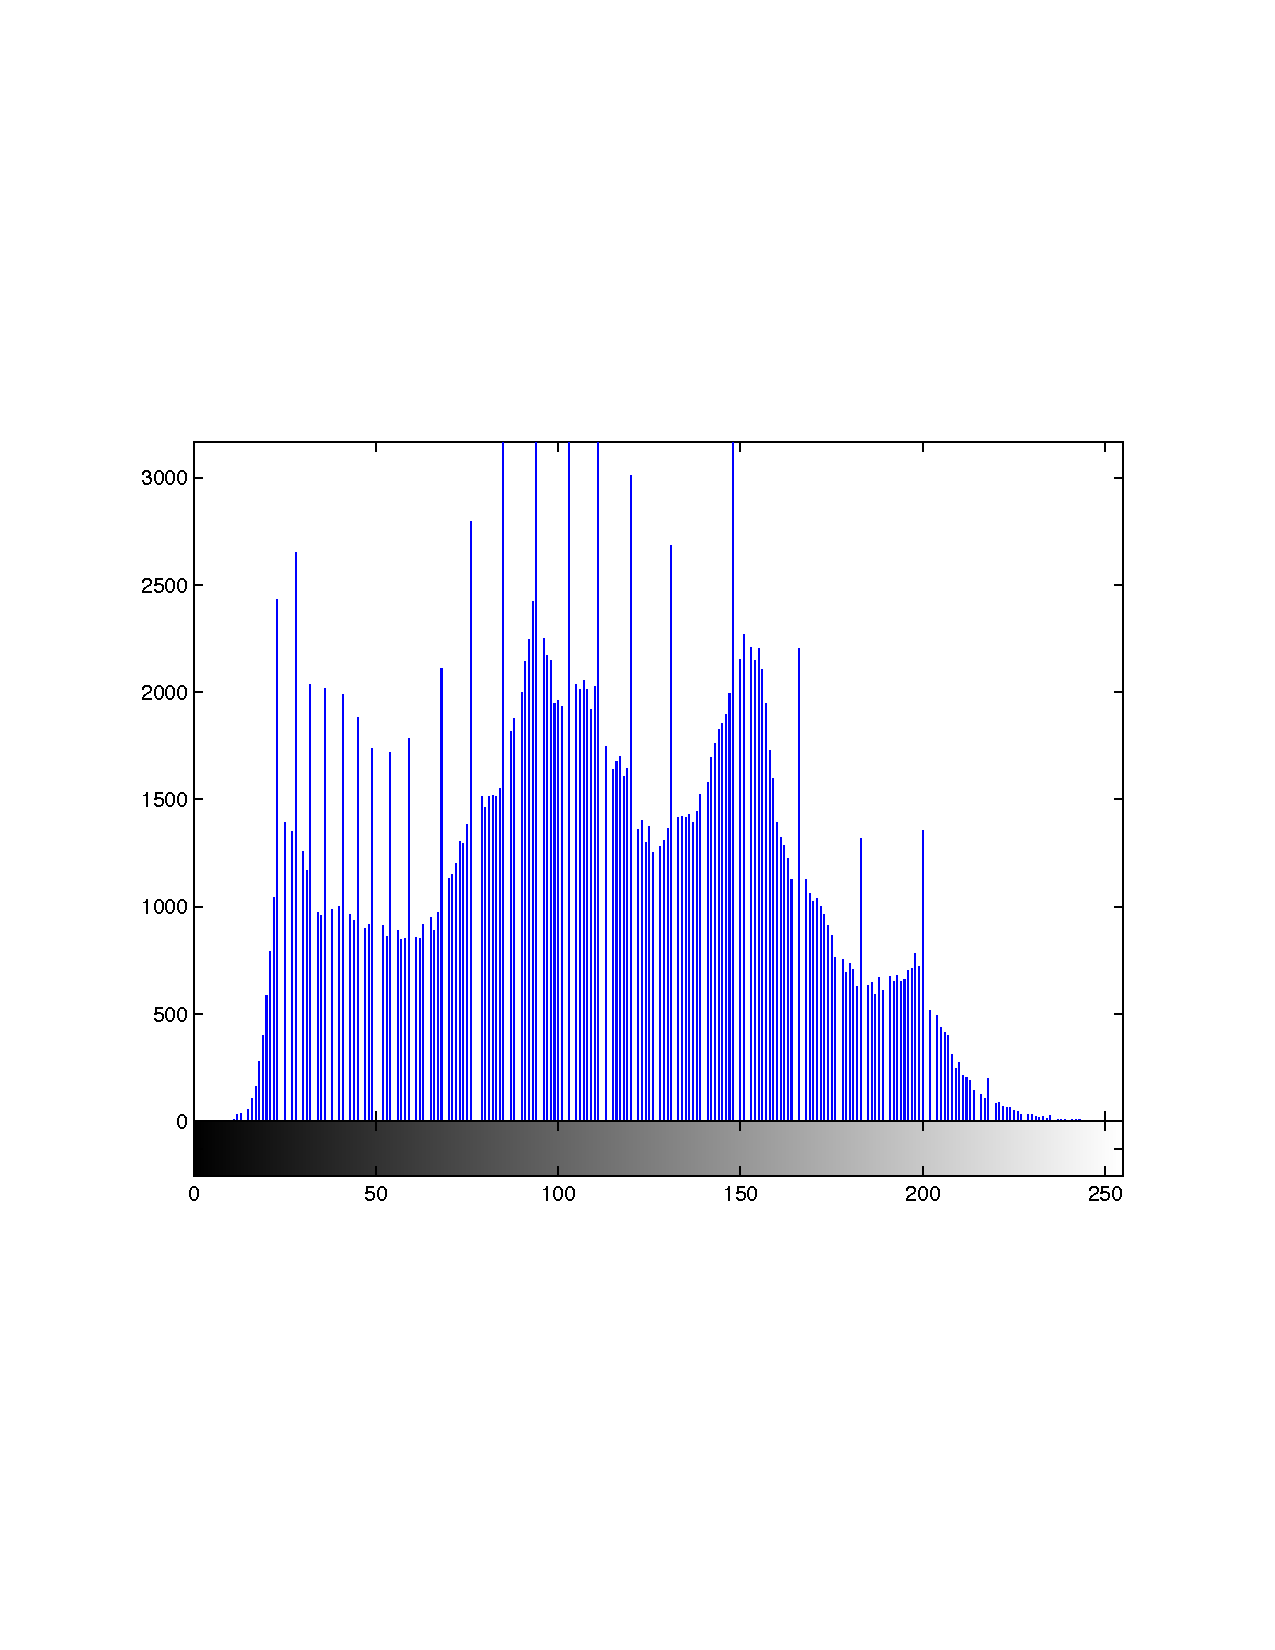
\includegraphics[width=\textwidth]{q4-b-orighist}
                \caption{Histogram of original image}
                \label{fig:bhe}
        \end{subfigure}%
        ~ %add desired spacing between images, e. g. ~, \quad, \qquad etc. 
          %(or a blank line to force the subfigure onto a new line)
        \begin{subfigure}[b]{0.3\textwidth}
                \centering
                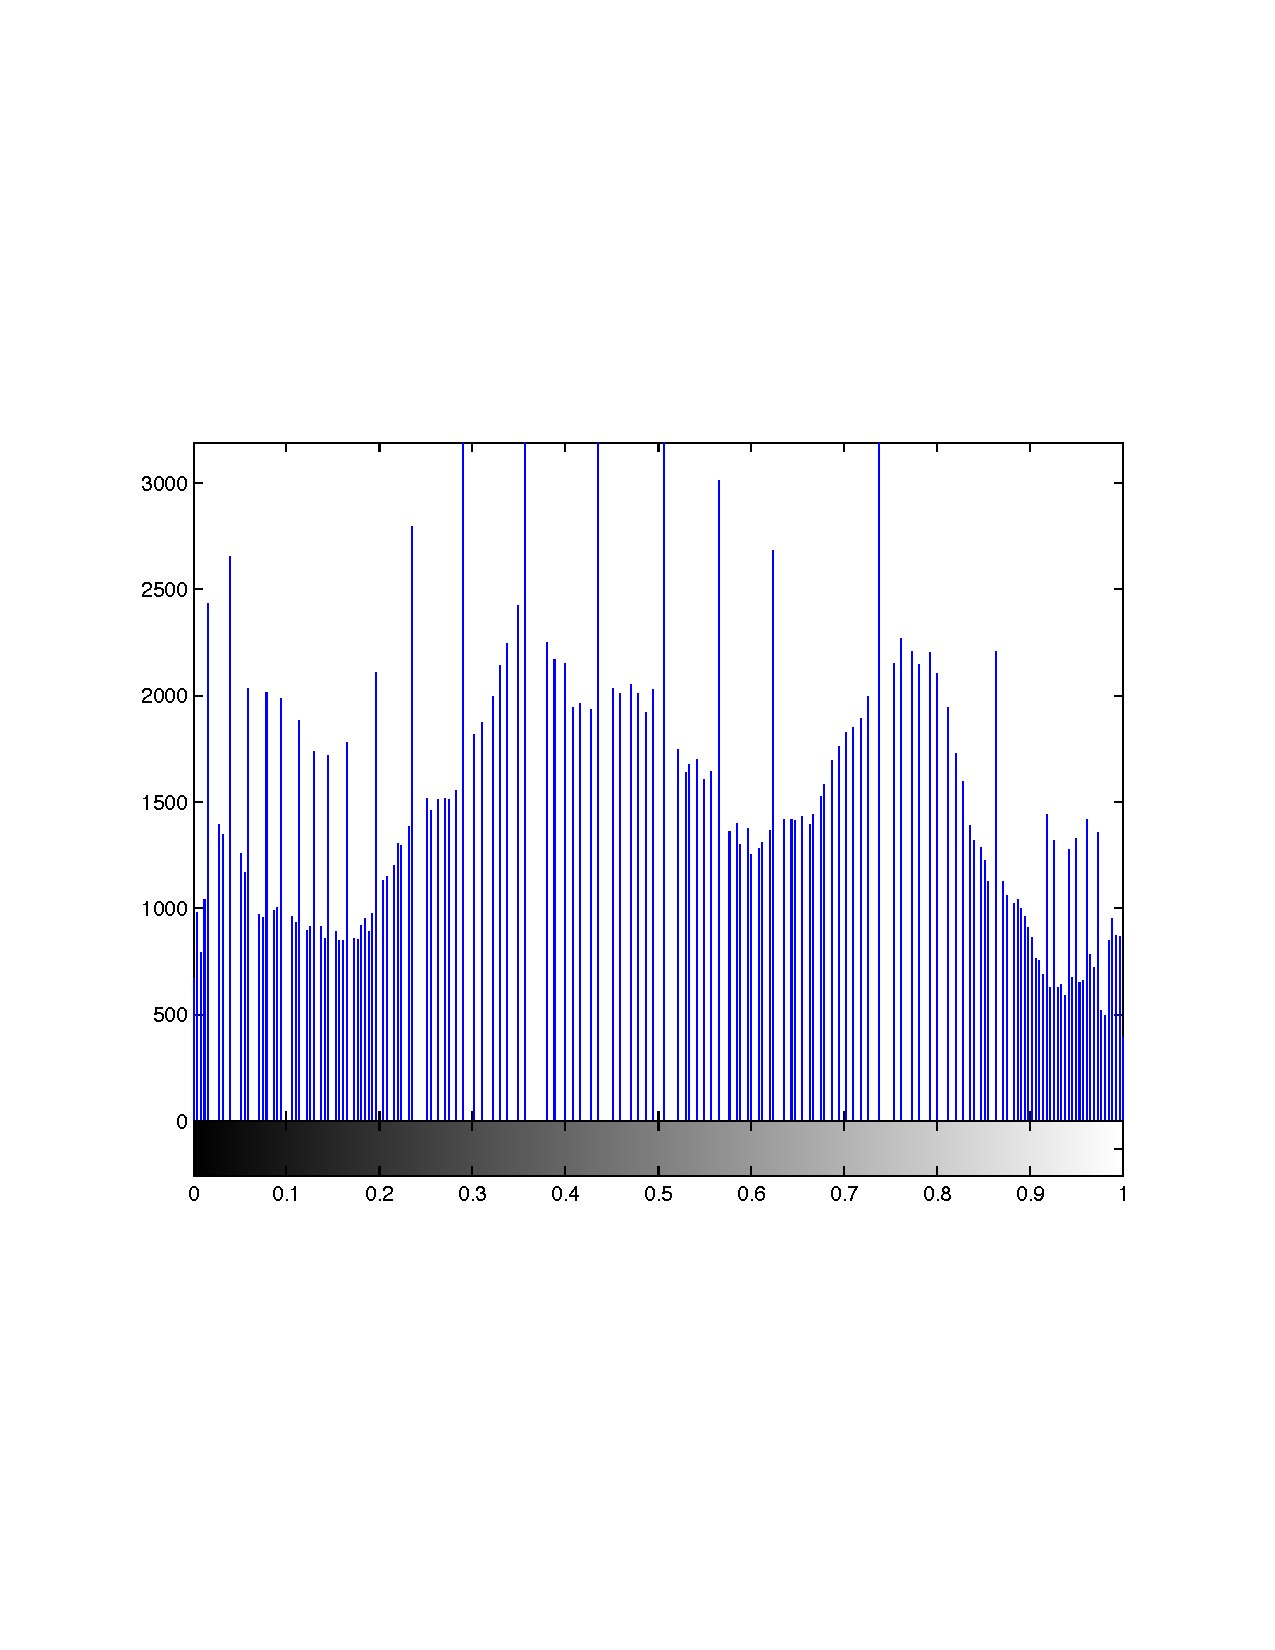
\includegraphics[width=\textwidth]{q4-b-thist}
                \caption{Equalised histogram}
                \label{fig:ahe}
        \end{subfigure}
        \caption{Results of applying histogram equalisation}
        \label{fig:441compare}
\end{figure}

\begin{figure}[ht]
        \centering
        \begin{subfigure}[b]{0.3\textwidth}
                \centering
                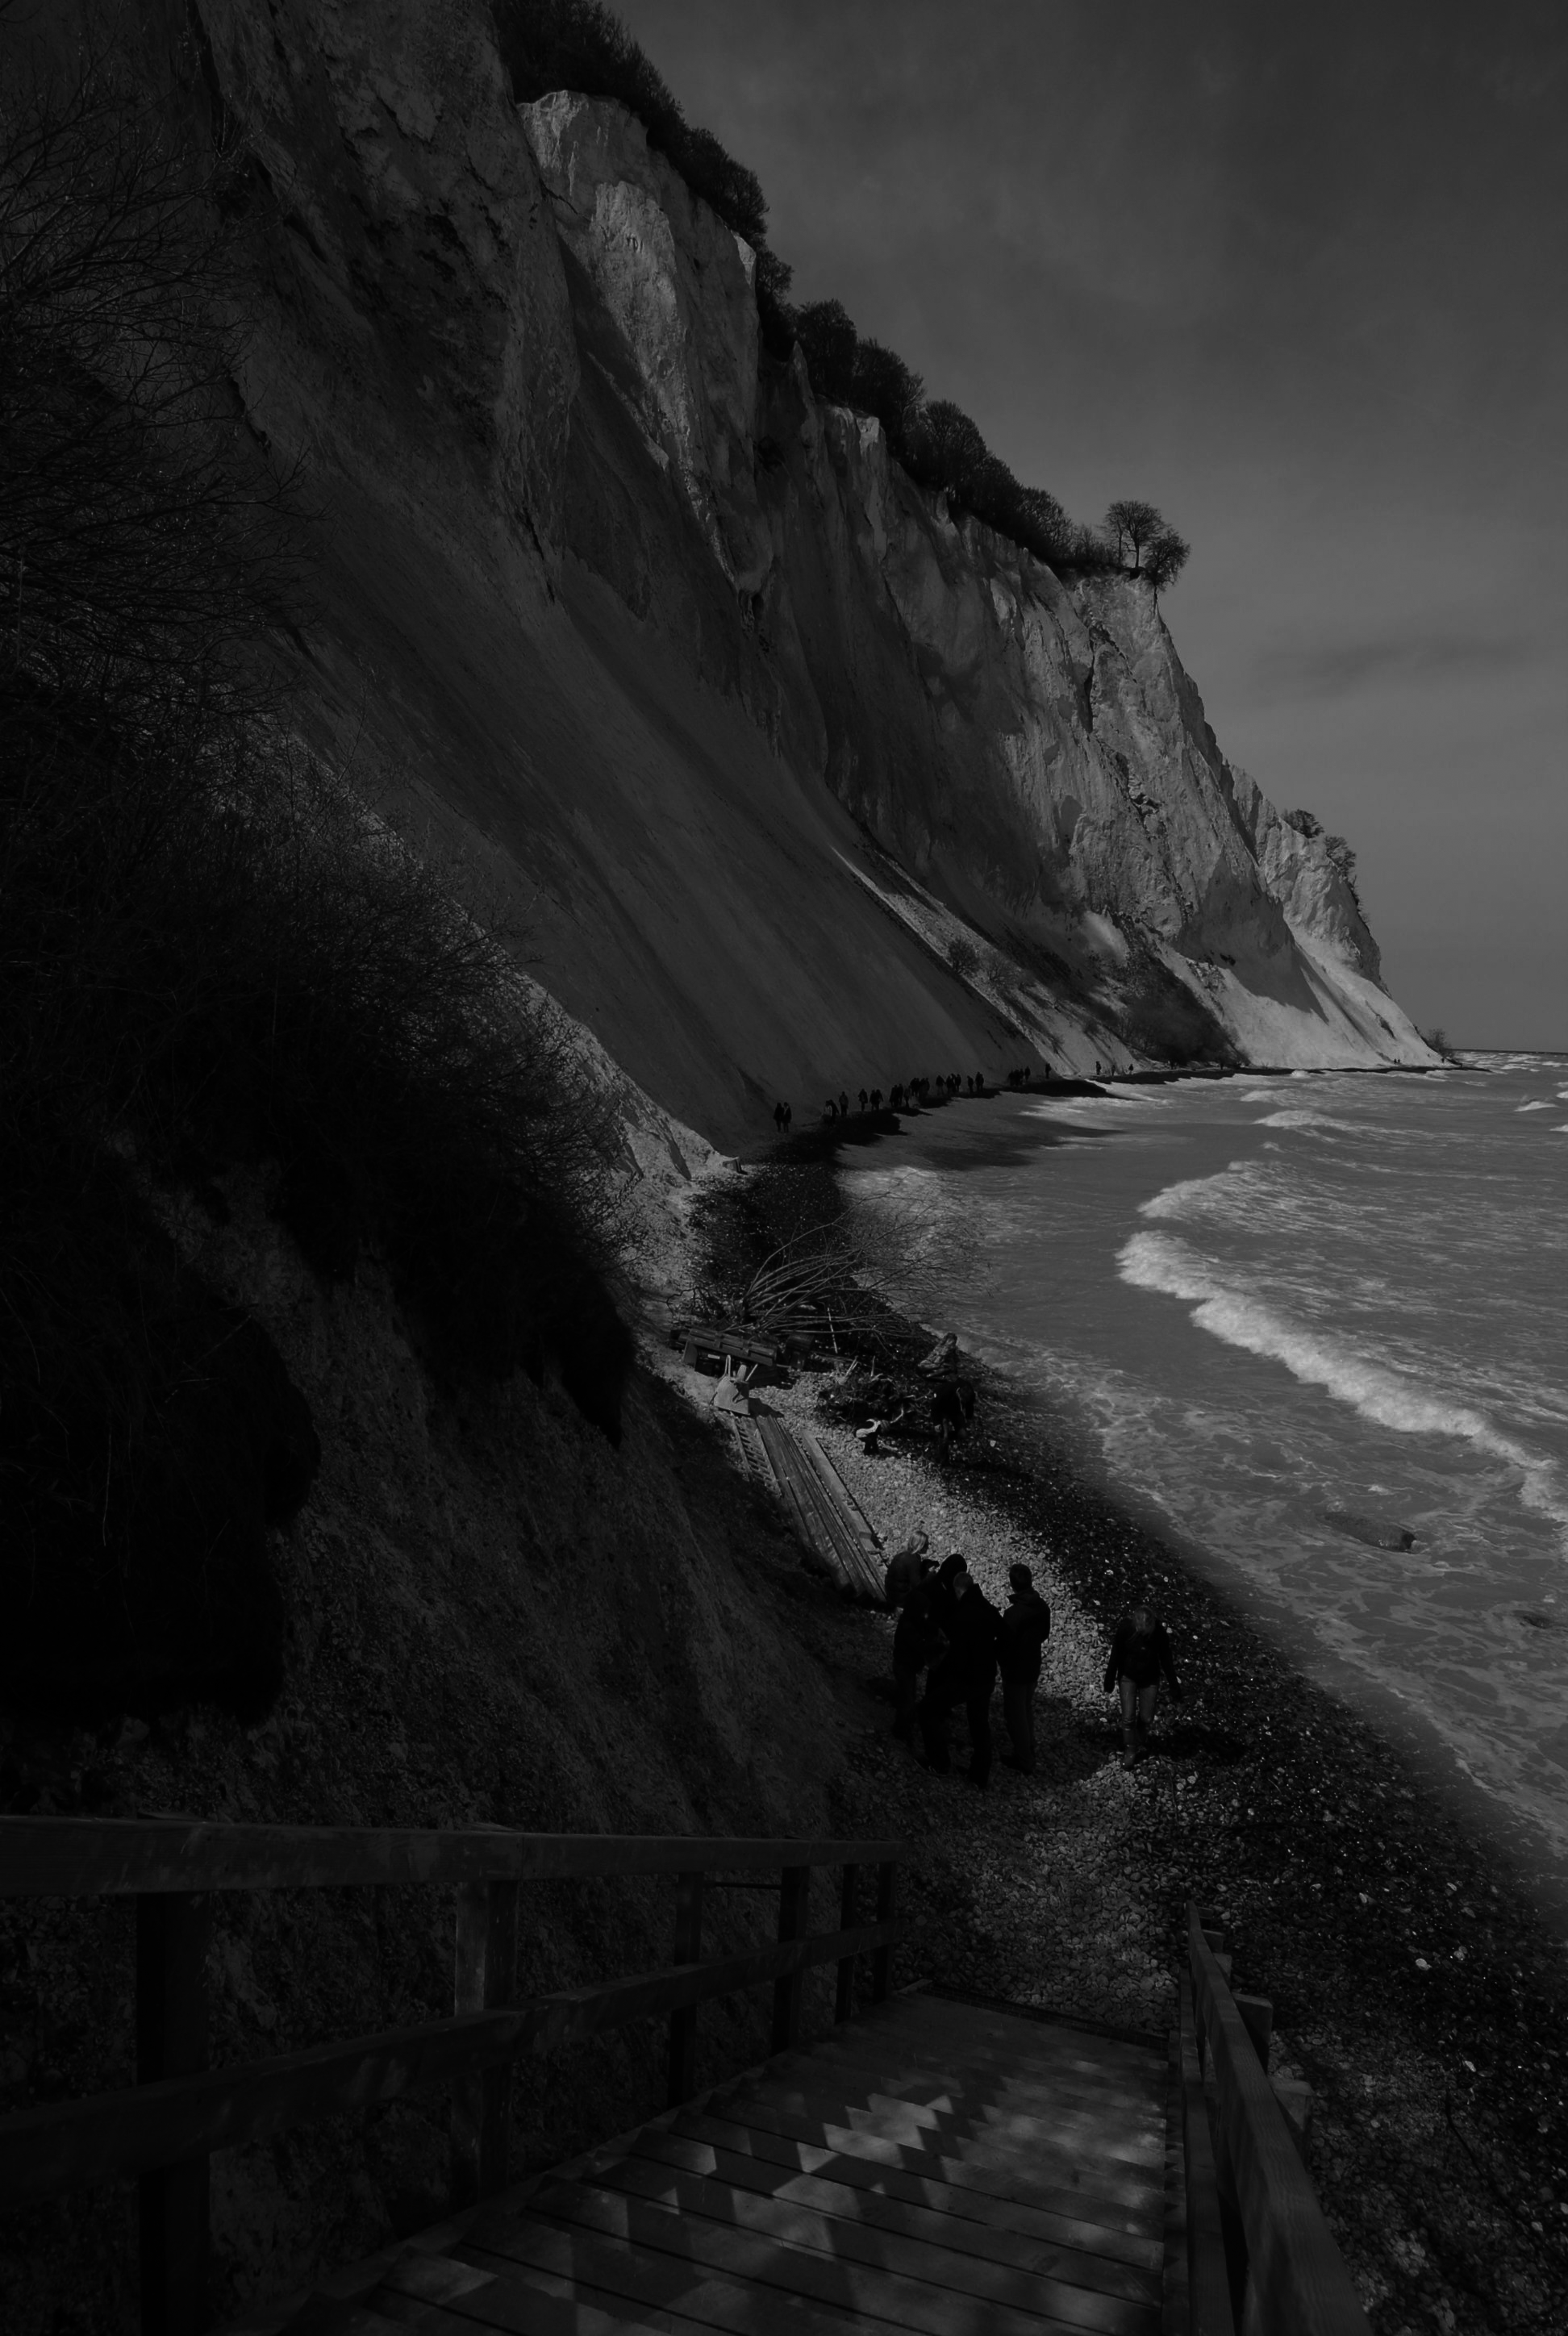
\includegraphics[width=\textwidth]{q4b-orig.png}
                \caption{Input image}
                \label{fig:be2}
        \end{subfigure}
        \begin{subfigure}[b]{0.3\textwidth}
                \centering
                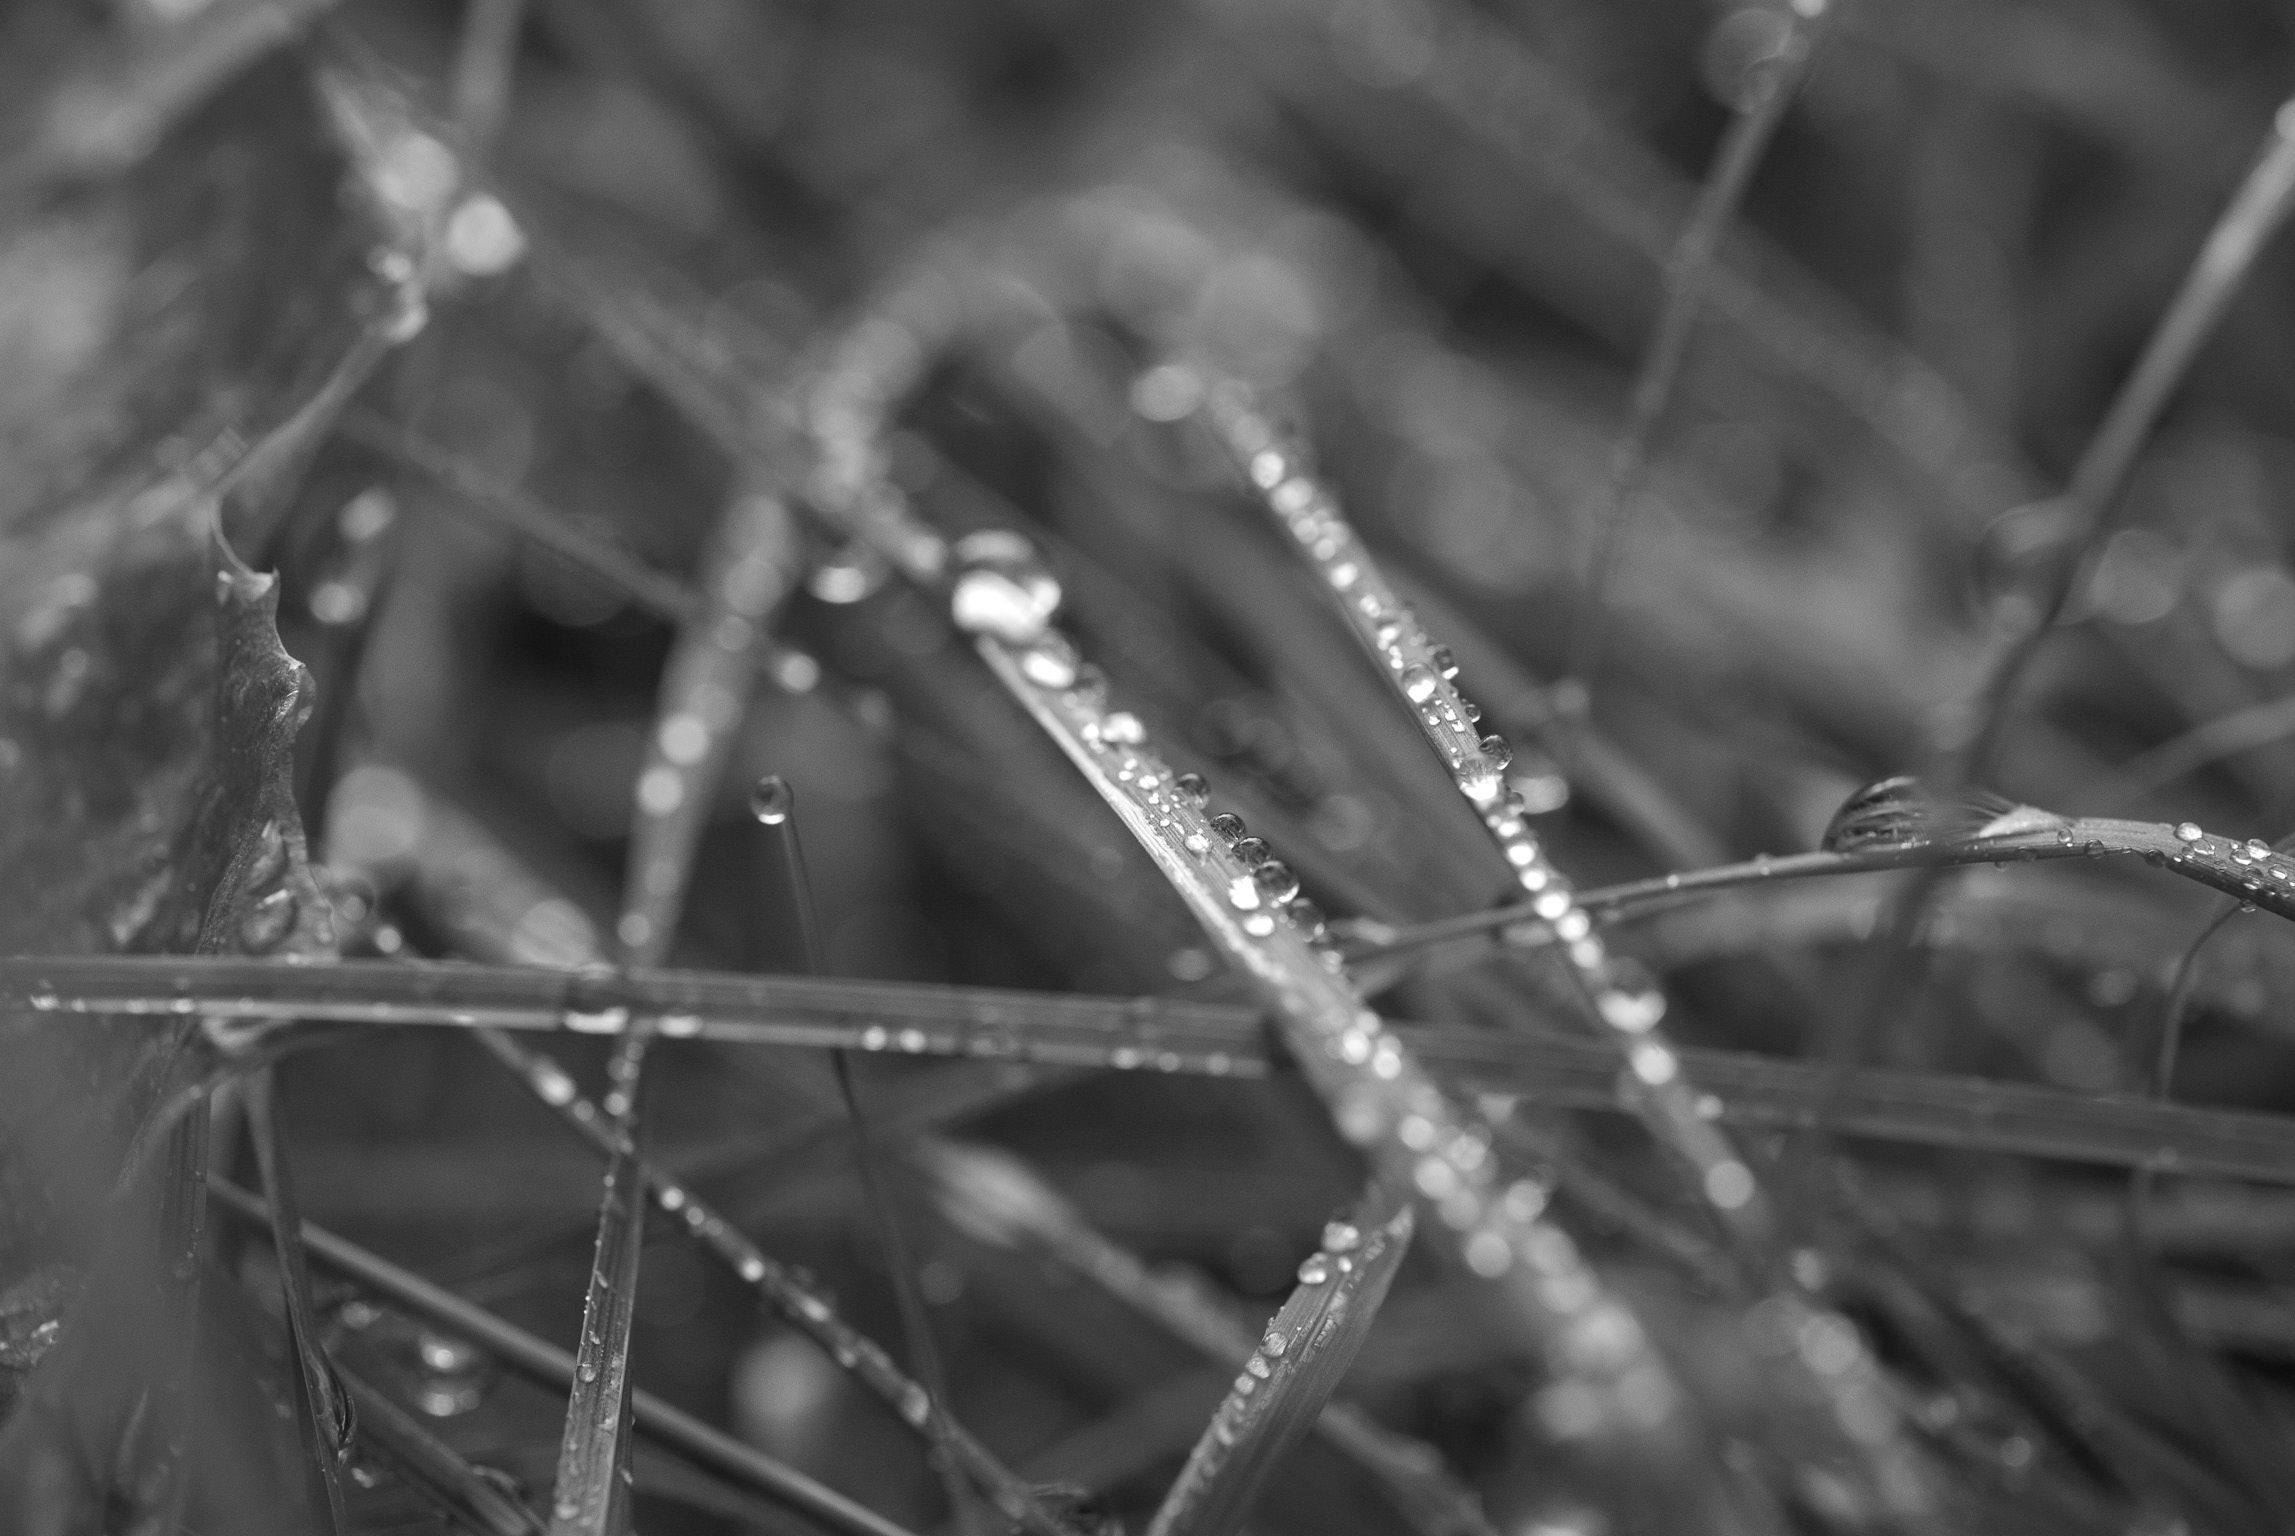
\includegraphics[width=\textwidth]{q4b-match.png}
                \caption{Specimen image}
                \label{fig:abe2}
        \end{subfigure}
        \begin{subfigure}[b]{0.3\textwidth}
                \centering
                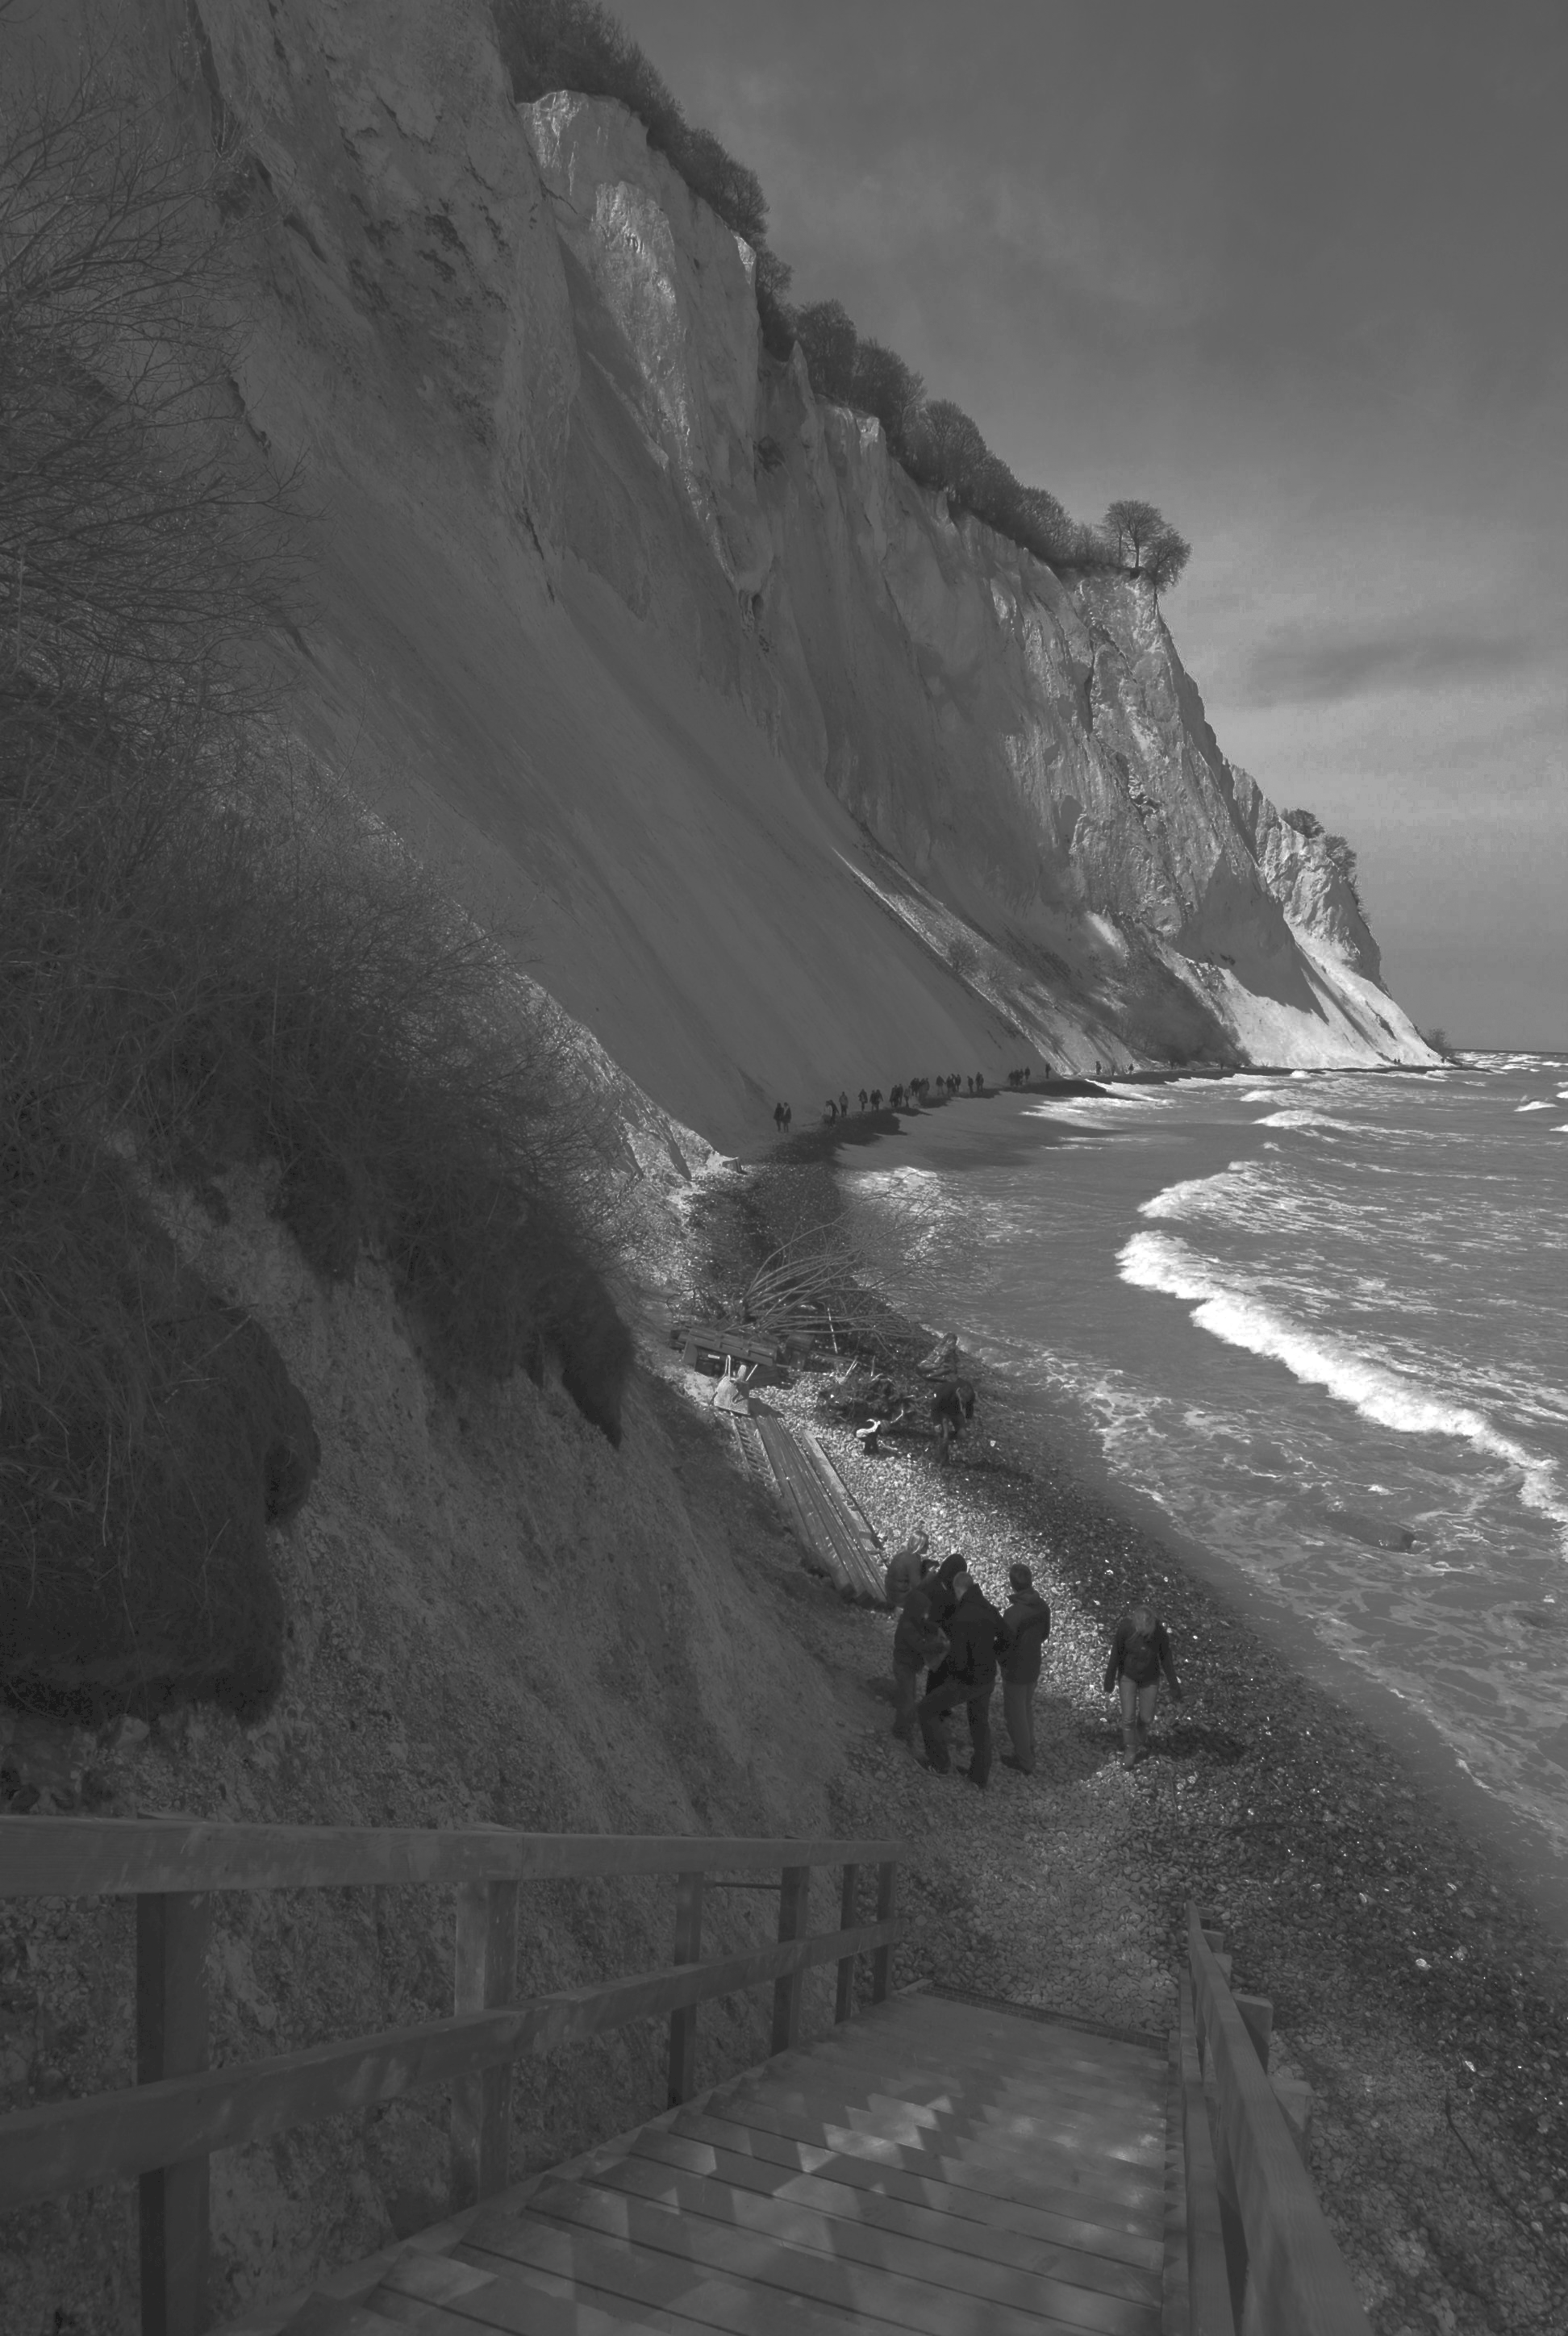
\includegraphics[width=\textwidth]{q4b-result.png}
                \caption{Image after matching}
                \label{fig:ae2}
        \end{subfigure}
        
        \begin{subfigure}[b]{0.3\textwidth}
                \centering
                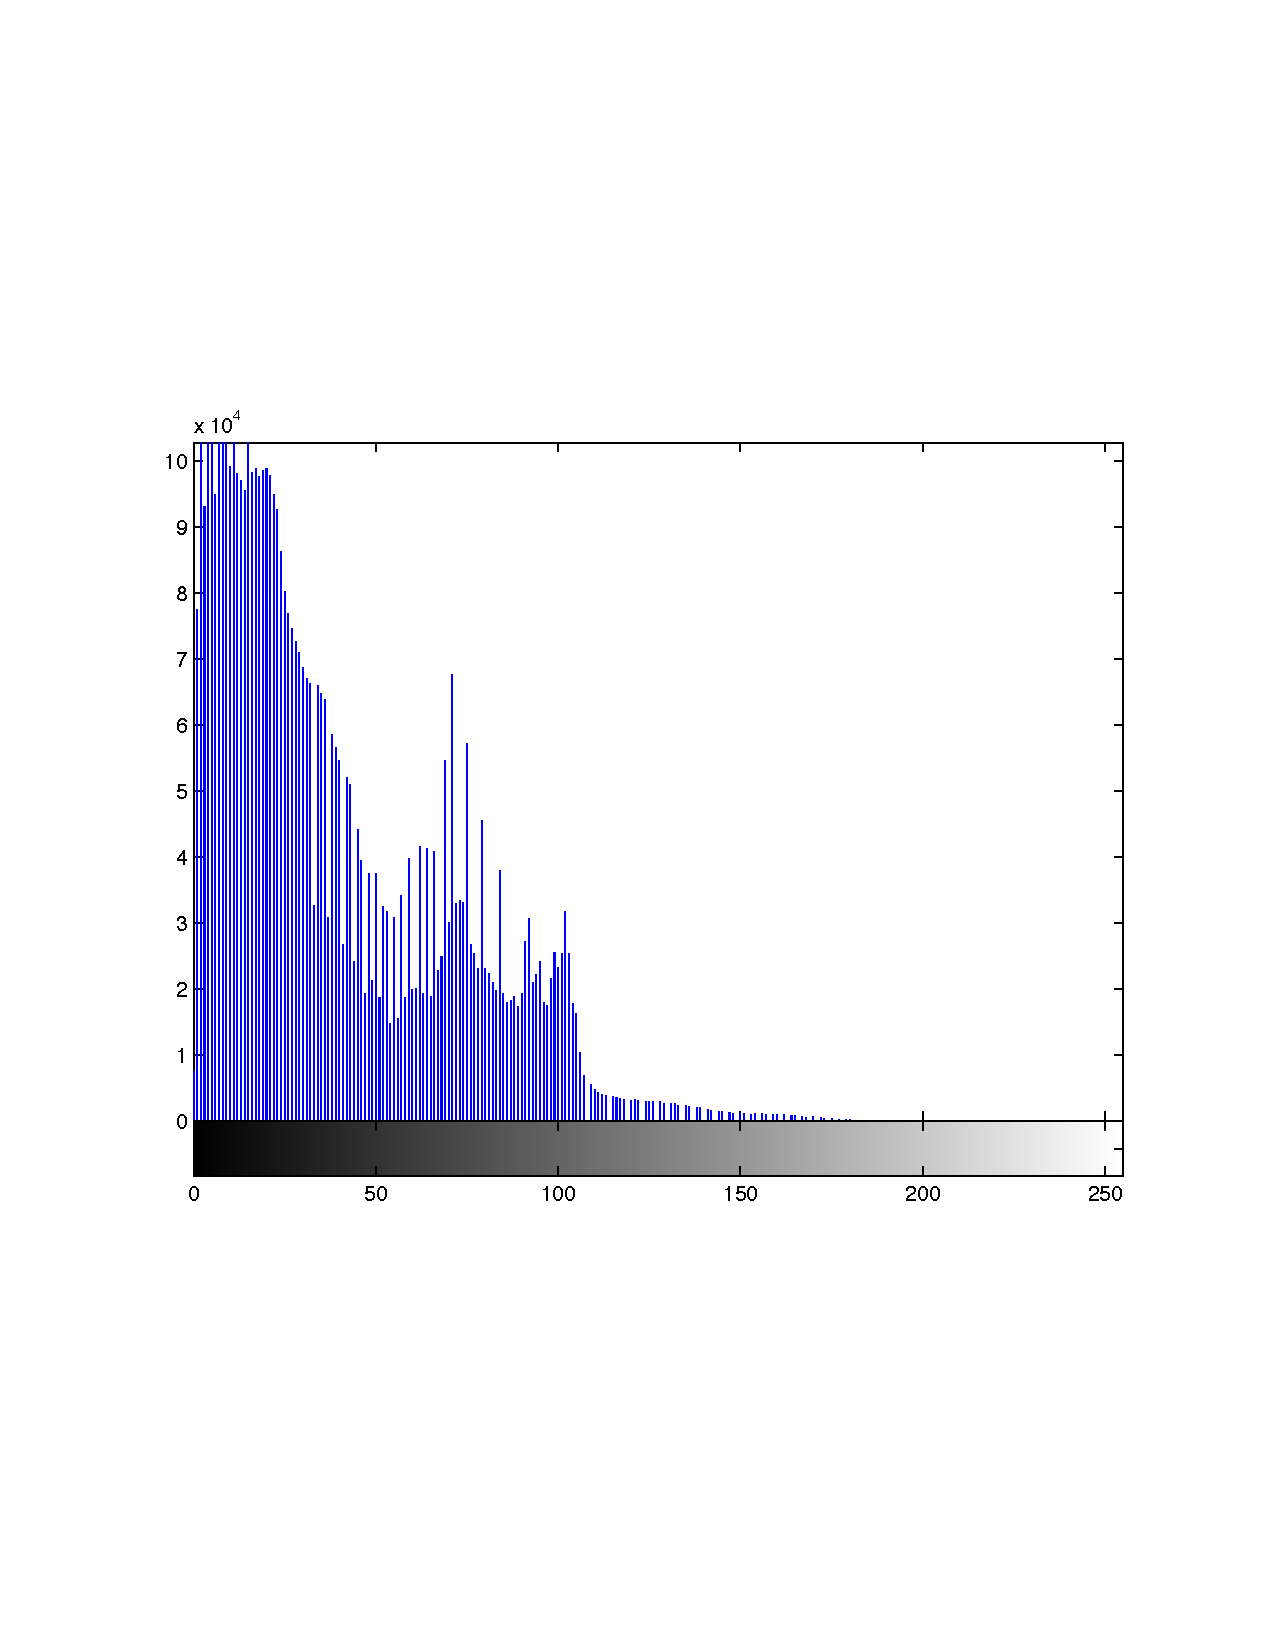
\includegraphics[width=\textwidth]{q4-c-orighist}
                \caption{Original histogram}
                \label{fig:bhe2}
        \end{subfigure}%
        \begin{subfigure}[b]{0.3\textwidth}
                \centering
                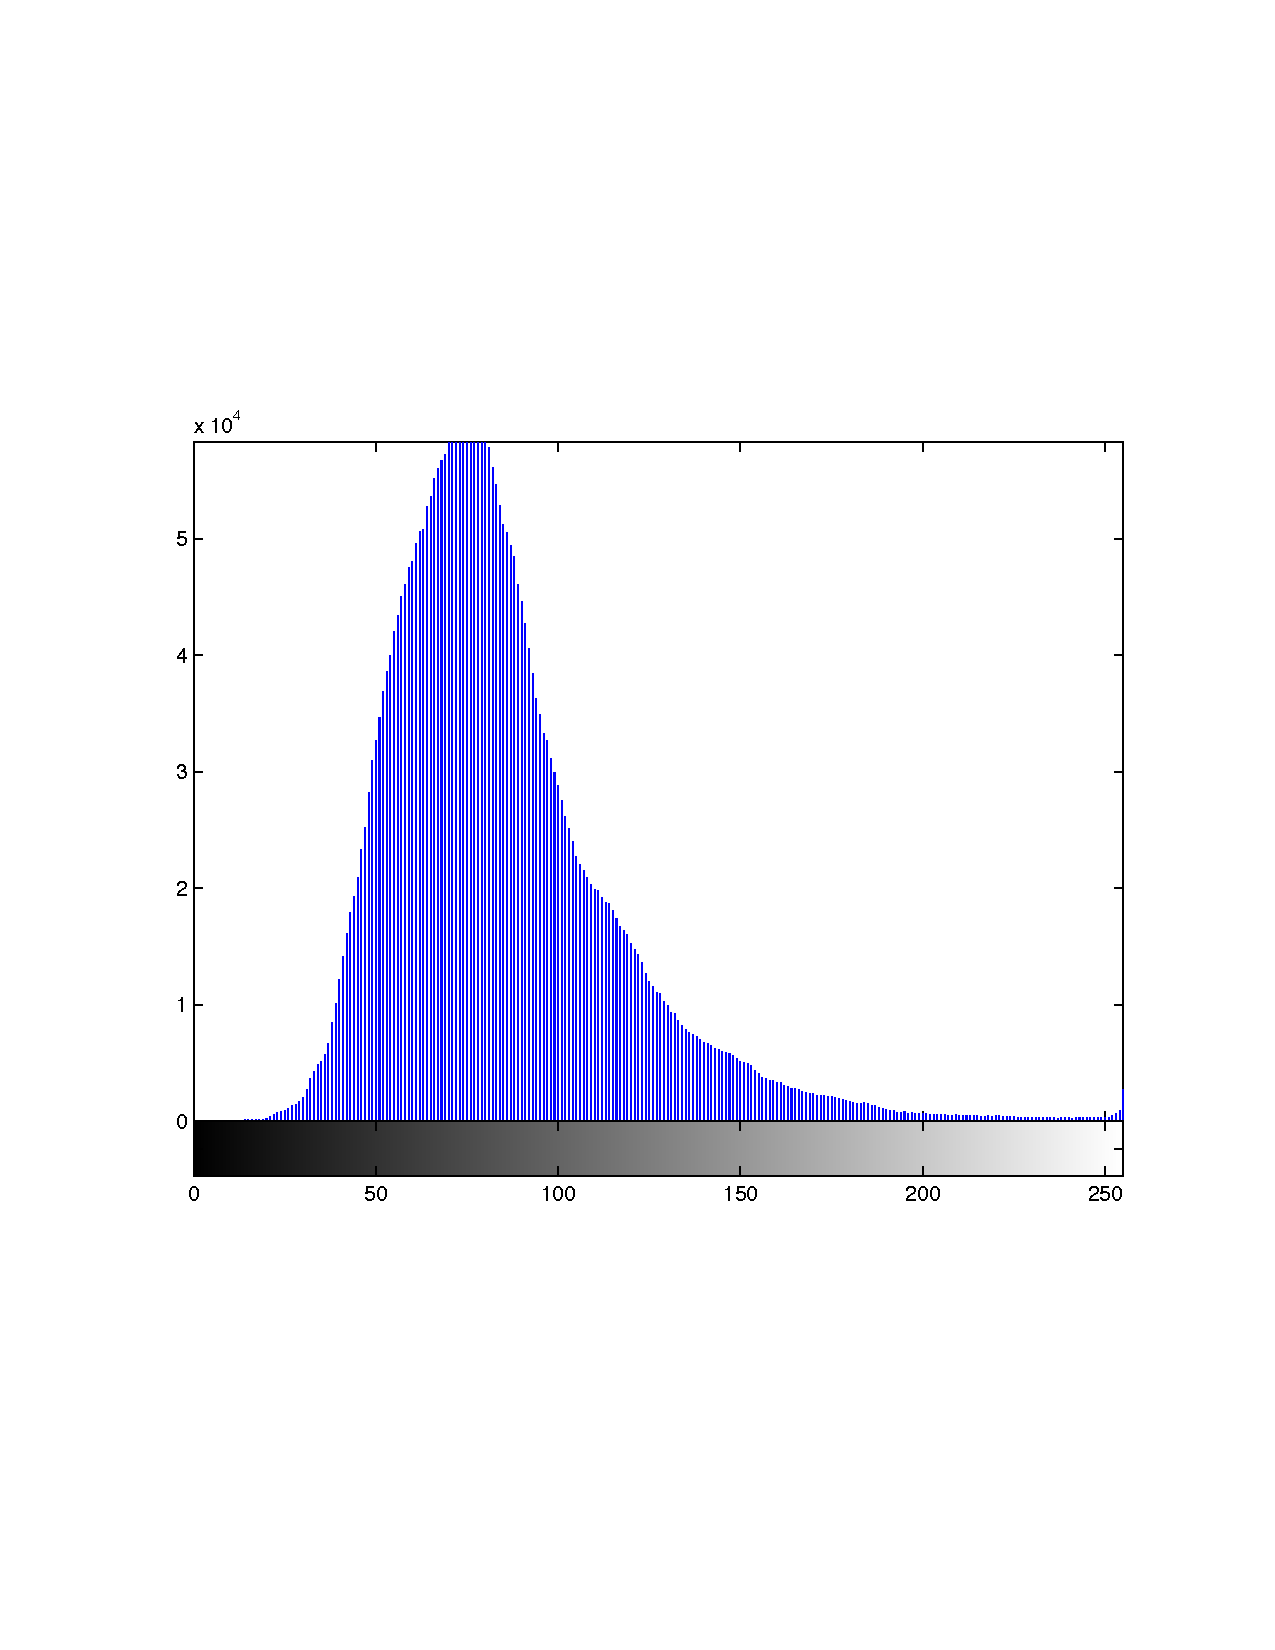
\includegraphics[width=\textwidth]{q4-c-spechist}
                \caption{Specimen histogram}
                \label{fig:bhe3}
        \end{subfigure}%
        ~ %add desired spacing between images, e. g. ~, \quad, \qquad etc. 
          %(or a blank line to force the subfigure onto a new line)
        \begin{subfigure}[b]{0.3\textwidth}
                \centering
                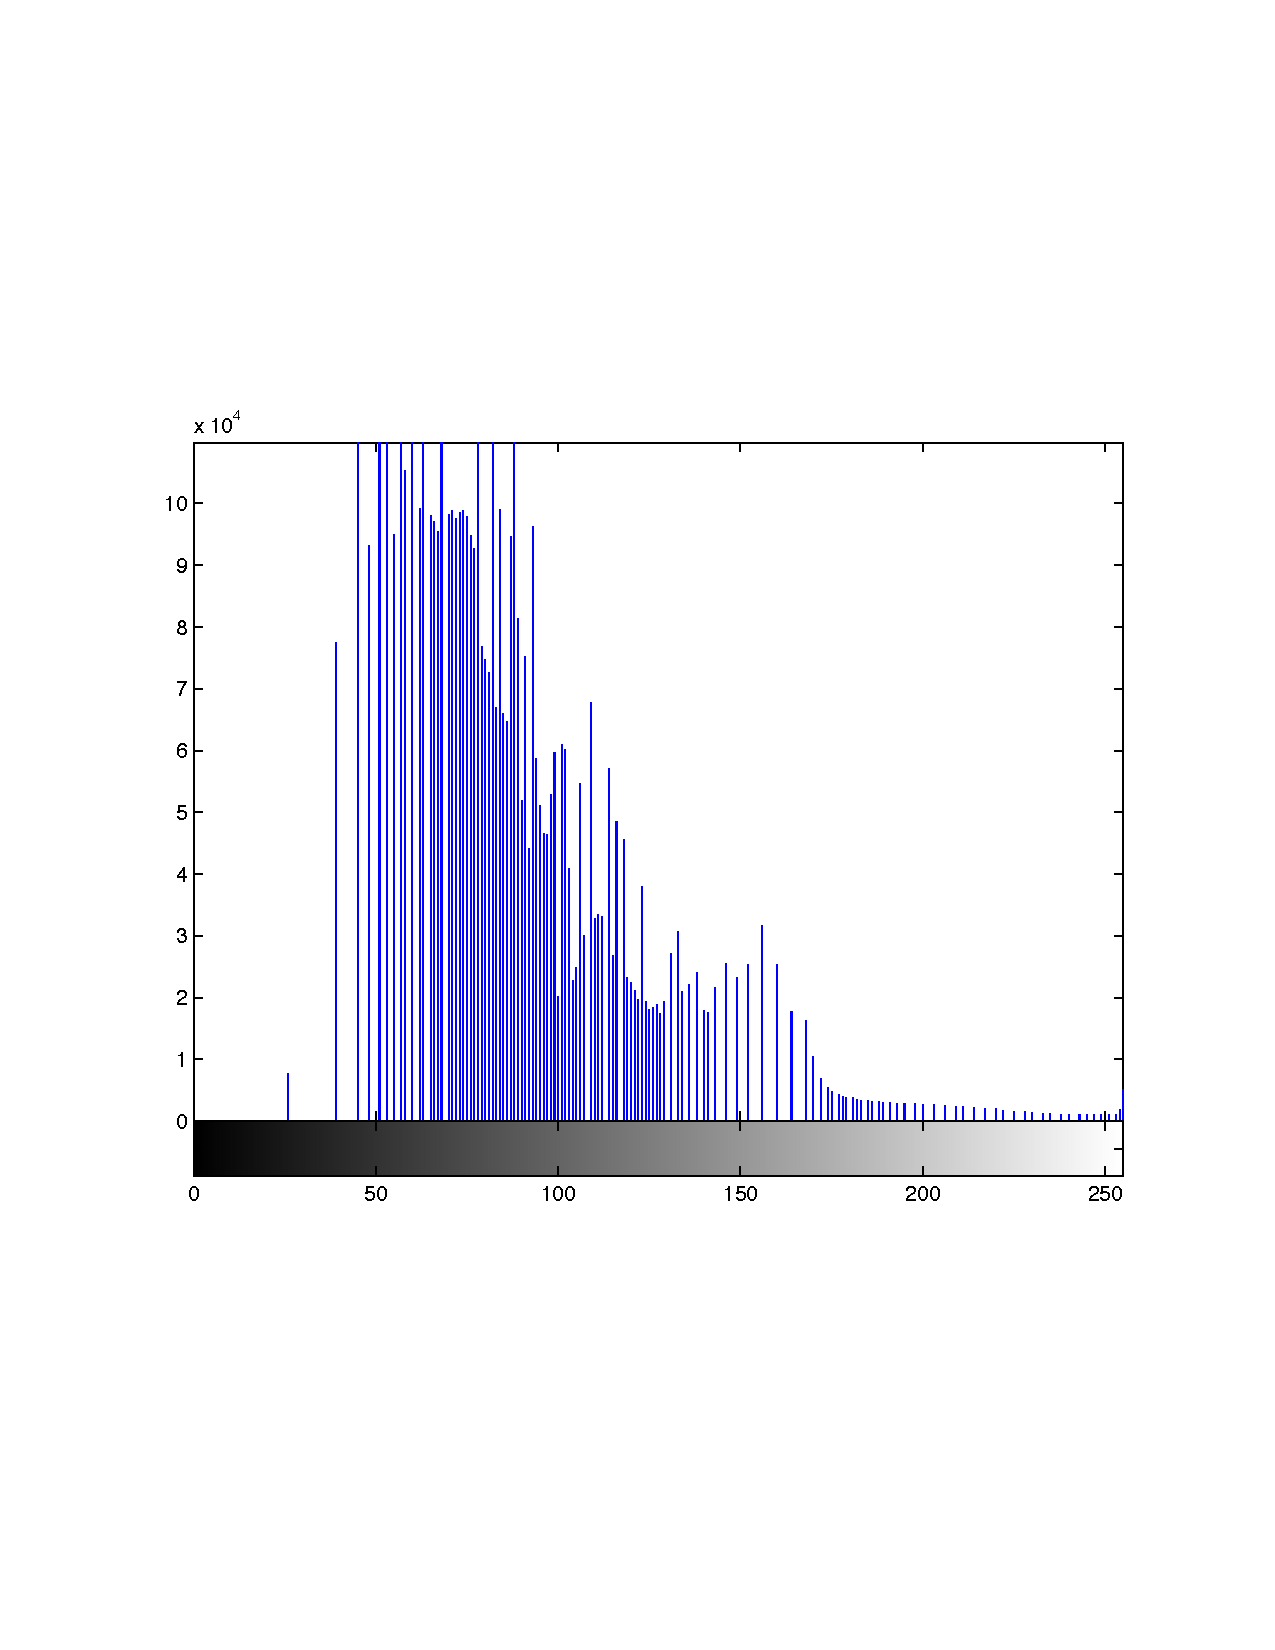
\includegraphics[width=\textwidth]{q4-c-thist}
                \caption{Matched histogram}
                \label{fig:ahe2}
        \end{subfigure}
        \caption{Results of applying histogram matching. Images taken by the author}
        \label{fig:442compare}
\end{figure}

\section*{Question 4.5 - RGB to HSI and back again} 

My implementation of RGB to HSI and the inverse are listed in appendices \ref{appendix-rgbhsi} and \ref{appendix-hsirgb}.


\clearpage
\appendix 
\section{Gammatool.m source} 
\label{appendix-gammatool} 
\lstinputlisting{gammatool.m}

\section{histogram\_equalise.m source} 
\label{appendix-hist-eq} 
\lstinputlisting{histogram_equalise.m}

\section{histogram\_match.m source} 
\label{appendix-hist-match} 
\lstinputlisting[language=Matlab]{histogram_match.m}

\section{RGBtoHSI.m}
\label{appendix-rgbhsi}
\lstinputlisting[language=Matlab]{RGBtoHSI.m}

\section{HSItoRGB.m}
\label{appendix-hsirgb}
\lstinputlisting[language=Matlab]{HSItoRGB.m}

\end{document} 
